\chapter{Marco teórico.} \label{cap:marco_teorico}

\mynote{Este capítulo sirve como una breve introducción a todos los métodos, conceptos y modelos considerados para el desarrollo de este trabajo.}

Todo proceso de clasificación de imágenes puede dividirse en los siguientes pasos:

\begin{itemize}
	\item Tratado inicial de las imágenes
	\item Extracción de características
	\item Tratamiento de datos
	\item Entrenamiento de modelo de clasificación
	\item Evaluación modelo de clasificación
\end{itemize}

\section{Extracción de características}
\label{section:Extracción de catacterísticas}

En este paso el objetivo es obtener información cuantitativa (numérica) de las muestras a partir de diversos métodos.\\ Por ejemplo, de una clasificación de números escritos a mano se pueden obtener características como el número de trazos, anchura del contorno, color, etc. Es decir, se obtienen una serie de propiedades informativas de la muestra para, después, entrenar el modelo de clasificación. 

Para este trabajo, se han utilizado los siguientes métodos:
\begin{itemize}
	\item Descriptores de Fourier
	\item Momentos de imagen (Momentos Hu)
	\item Descriptores locales binarios (\textit{Local Binary Patterns})
	\item Histograma de gradientes
	\item *Método propio
\end{itemize}

\subsection{Momentos de imagen.}

Los momentos de imagen son un promedio de las intensidades de una imagen binaria. La convención habitual define un momento \(M\) para una imagen binaria \(B\) de la siguiente forma:

\begin{equation}
	\label{eqn:momento}
	M_{ij} = \sum_{x}^{} \sum_{y}^{} x^{i} y^{j} B(x,y)
\end{equation}

Utilizando la ecuación \ref{eqn:momento}, se pueden obtener características la imagen como los centroides:
\begin{equation}
	\label{eqn:momentos_x_centroide}
	\overline{x} = \dfrac{M_{10}}{M_{00}}
\end{equation}
\begin{equation}
	\label{eqn:momentos_y_centroide}
	\overline{y} = \dfrac{M_{01}}{M_{00}}
\end{equation}

Sin embargo, aplicando una transformación a la ecuación \ref{eqn:momento}, se pueden obtener momentos invariantes a la traslación:

\begin{equation}
	\label{eqn:momentos_central}
	\mu_{i,j} = \sum_{x} \sum_{y} (x-\overline{x})^{i} (y-\overline{y})^{j} I(x,y)
\end{equation}

A la ecuación \ref{eqn:momentos_central} se la conoce como \textbf{momentos centrales}.

Además, aplicando otra transformación se pueden obtener momentos invariantes al escalado también:

\begin{equation}
	\label{eqn:momento_normalizado}
	\eta_{i,j} = \dfrac{\mu_{i,j}}{\mu_{00}^{\dfrac{i+j}{2}+1}}
\end{equation}

La fórmula \ref{eqn:momento_normalizado} se conoce como \textbf{momento centralizado}.

\subsubsection{Momentos de Hu}

Los momentos de Hu \cite{1057692} son un un conjunto de siete fórmulas obtenidas a partir de los momentos centralizados que permiten obtener siete momentos invariantes tanto a traslación, rotación, escalado y volteado (el séptimo momento es el invariante a volteado, cambiando de signo cuando la imagen es reflejada).


\begin{equation}
	\label{eqn:hu_momentos}
	\begin{split}
		M_{1} = \eta_{20} + \eta_{02} \\
		M_{2} = (\eta_{20}-\eta_{02})^{2} + 4\eta_{11}^{2} \\
		M_{3} = (\eta_{30}-3\eta_{12})^{2} + (3\eta_{21}-\eta_{03})^{2} \\
		M_{4} = (\eta_{30}+\eta_{12})^{2} + (\eta_{21}+\eta_{03})^{2} \\
		M_{5} & = (\eta_{30}-3\eta_{12})(\eta_{30}+\eta_{12})[(\eta_{30}+\eta_{12})^{2}-3(\eta_{21}+3\eta_{03})^{2}] \\
		& +(3\eta_{21}-\eta_{03})(\eta_{21}+\eta_{03})[3(\eta_{30}+\eta_{12})^{2}-(\eta_{21}+\eta_{03})^{2}] \\
		M_{6} & = (\eta_{20}-\eta_{02}[(\eta_{30}+\eta_{12})^{2}-(\eta_{21}+\eta_{03})^{2}] \\
		& +4\eta_{11}(\eta_{30}+\eta_{12})(\eta_{21}+\eta_{03}) \\
		M_{7} = (3\eta_{21}-\eta_{03})(\eta_{30}+\eta_{12})[(\eta_{30}+\eta_{12})^{2}-3(\eta_{21}+3\eta_{03})^{2}] \\
		& -(\eta_{30}-3\eta_{12})(\eta_{21}+\eta_{03})[3(\eta_{30}+\eta_{12})^{2}-(\eta_{21}+\eta_{03})^{2}]
	\end{split}
\end{equation}

A partir de \ref{eqn:hu_momentos}, se pueden obtener siete características númericas.

\pagebreak
\subsection{Histograma de gradientes}

El histograma de gradientes \cite{osti_6007283} es una técnica de extración de características muy utilizada en la detección de objetos.

A partir de una imagen binaria de dimensiones $ nxm $, se calculan los gradientes de intensidad, así como la magnitud y el ángulo:

\begin{equation}
	\label{eqn:hog_GxGy}
	\begin{split}		
		G_{x} = B(x+1,y) - B(x,y) \\
		G_{y} = B(x,y+1) - B(x,y)
	\end{split}
\end{equation}

La ecuación \ref{eqn:hog_GxGy} determina los gradientes de la imagen binaria \(B\). Tanto \(G_{x}\) como \(G_{y}\) son dos imágenes binarias con la información de gradientes en ejes X e Y, respectivamente. 
A partir de la ecuación \ref{eqn:hog_GxGy}, se obtienen las magnitudes y ángulos:

\begin{equation}
	\label{eqn:hog_mag}
	Mag_{(x,y)} (\mu)= \sqrt{G_{x}^{2}+G_{y}^{2}}
\end{equation}

\begin{equation}
	\label{eqn:hog_angulo}
	Ang_{(x,y)} (\theta) = \lvert tan^{-1}(\dfrac{G_{y}}{G_{x}})\lvert
\end{equation}

Tanto la ecuación \ref{eqn:hog_mag} como \ref{eqn:hog_angulo} representan imágenes binarias.

El siguiente paso consiste en dividir las imágenes de magnitud y ángulos en $ N $ cuadrículas, pudiendo ser $ N = 1 $ (una única cuadrícula).

Para cada cuadrícula se representa un histograma de 9 posiciones, con cada posición en el rango $ [\theta,\theta+\delta\theta) $. Convencionalmente, se suele utilizar $\delta\theta = 20^{\circ}$ . De esta forma se obtiene el siguiente histograma $ H_{N}$:

\begin{table}[htb]
	\centering
	\caption{Histograma de gradientes, tabla ejemplo}
	\label{tab:hog_histograma_tabla}
	\begin{tabular}{|c||c|c|c|c|c|c|c|c|c|}
		\hline
		Magnitud &    &    &    &    &    &     &     &     &     \\ \hline
		Ángulo   & 0  & 20 & 40 & 60 & 80 & 100 & 120 & 140 & 160 \\ \hline
	\end{tabular}
\end{table}

A cada intervalo angular y de magnitud, se le denomina $ \theta_{j} $ y $ \mu_{j} $, respectivamente, para $ j\:\epsilon\:[0,8]$ .

De tal forma, si en la cuadrícula $ N_{i} $ existe un $\theta_{x,y}$ que pertenece al rango $ [\theta,\theta+\delta\theta j) $, para $ j\:\epsilon\:[0,8]$, se determina que $ \mu_{j} = \mu_{x,y} + \mu_{j}$.

\begin{equation}
	\label{eqn:hog_sum_magnitudes}
	\mu_{j} = \sum{\mu_{x,y}} \iff \theta_{x,y}\:\epsilon\:[\theta,\theta+\delta\theta \cdot j)
\end{equation}

Existen casos en los que $\theta_{x,y} > 160^{\circ}$, entonces $\mu_{x,y}$ contribuye tanto a $ 0^{\circ} $ como a $160^{\circ}$.

\begin{equation}
	\setlength{\jot}{14pt}
	\label{eqn:hog_angulo_mayor_de_160}
	\begin{split}
		\dfrac{180-\theta_{x,y}}{20}\cdot \mu_{x,y}\:\implies\: [160,180) \\
		\left(1-\dfrac{180-\theta_{x,y}}{20}\right)\cdot \mu_{x,y}\:\implies\: [0,20)
	\end{split}	
\end{equation}

El último paso consiste en normalizar el histograma:

\begin{equation}
	\label{eqn:hog_histograma_normalizacion}
	\mu_{j} = \dfrac{\mu_{j}}{max\:(\mu_{j})}
\end{equation}

Tras la aplicación de \ref{eqn:hog_histograma_normalizacion}, se tienen $ 9\cdot N$ características, siendo $ N $ el número de cuadrículas.

\pagebreak
\subsection{Patrones locales binarios}

También conocido por sus siglas del inglés \textbf{LBP} (del inglés, \textit{Local Binary Patterns}), este método propuesto en la decada de 1990 \cite{572934} permite extraer un histograma de 256 características de una muestra.

\begin{figure}[H]
	\centering
	\captionsetup{justification=centering}
	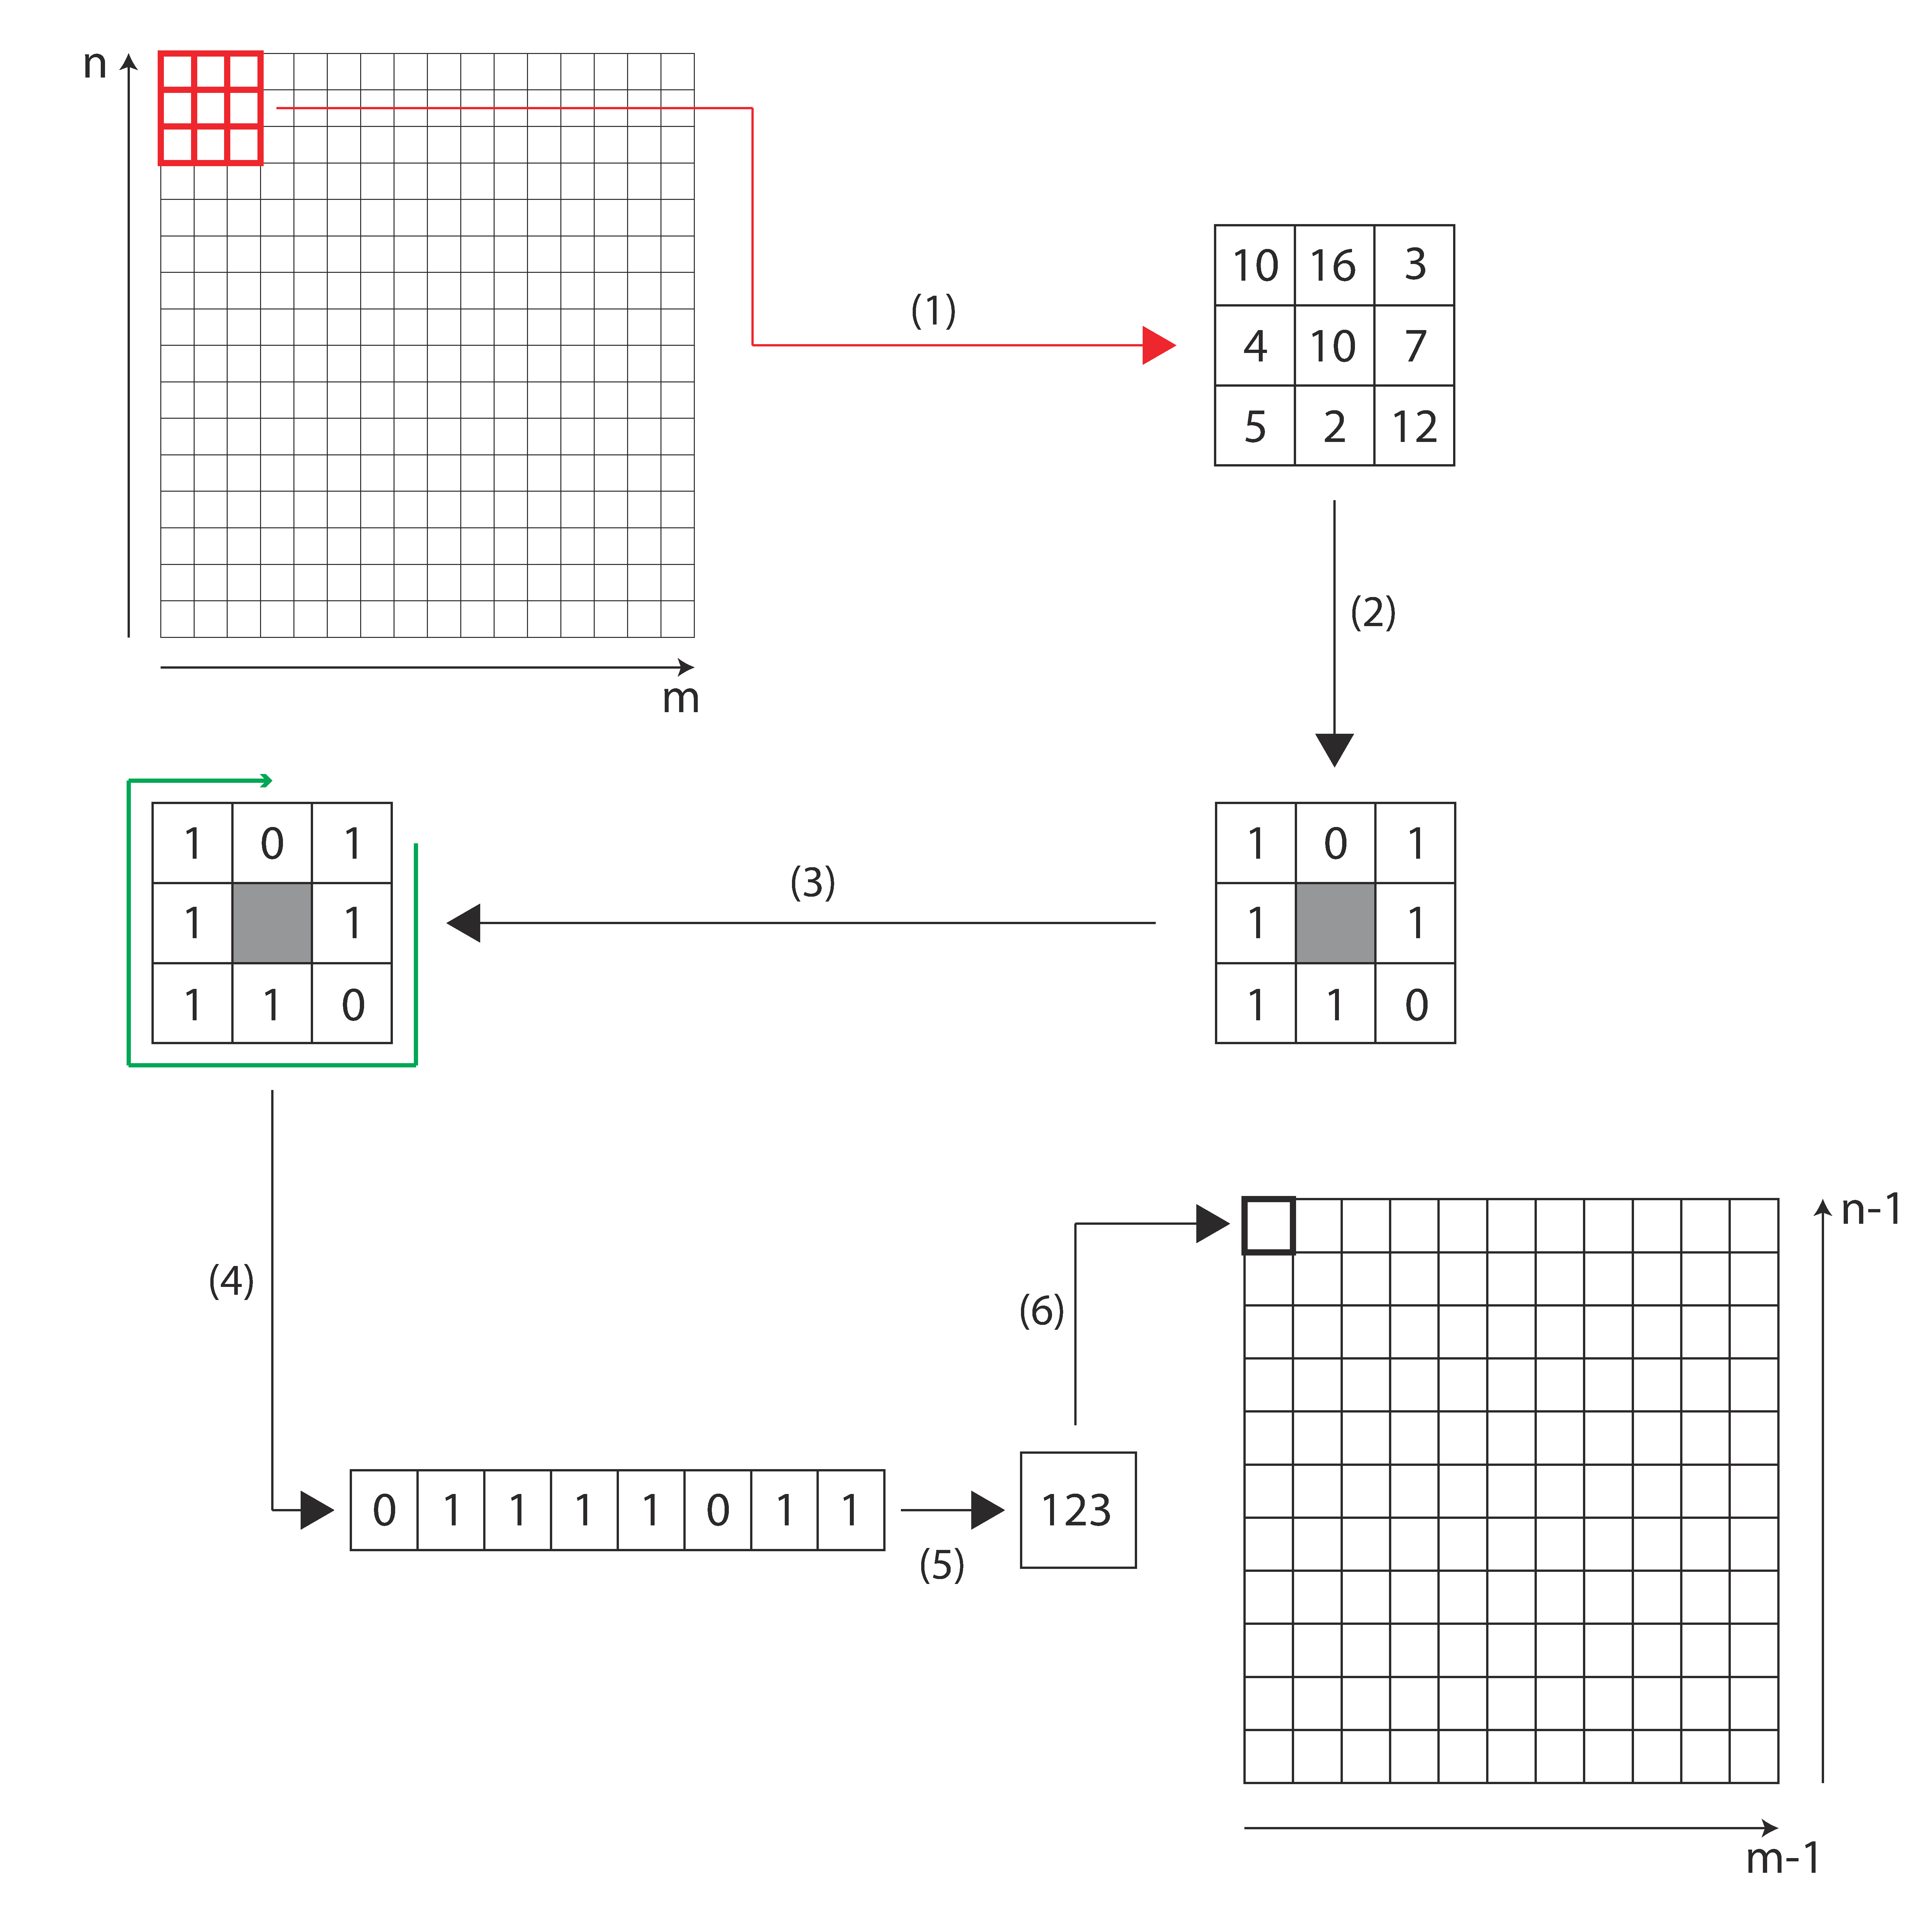
\includegraphics[width=\textwidth]{imagenes/marco_teorico/LBP/LBP_diagrama.pdf}
	\caption{Esquema método LBP}	
	\label{fig:LBP_diagrama}
\end{figure}

La figura \ref{fig:LBP_diagrama} muestra un esquematizado resumen del proceso de extración de características por este método.

La imagen original es tratada como una matriz de dimensiones $ n(filas) x\: m(columnas) $. A partir de esta, se extraen submatrices de dimensiones $3x3$ y se comienza el análisis de datos.

En la nueva submatriz, la posición central es comparada con las exteriores. Si, para una posición exterior, el valor central es menor o igual, se asigna a esta posición un valor 1. De ser mayor, se asigna un 0.

La nueva matriz binaria es tratada como un número binario de 8 dígitos, consisitiendo el siguiente paso en obtener el equivalente en base diez. Este último valor es almacenado en una nueva matriz de dimensiones $(n-1)x(m-1)$.

Realizando este proceso para toda la imagen original se tiene un conjunto de datos a partir de los cuales obtener el histograma sobre el que se basa el método \textbf{LBP}.

Teóricamente, el número máximo de características extraibles es 256 (ver \ref{eqn:LBP_rango}), pero pueden agruparse por rangos obteniendo grupos de características. Esta última opción es dependiente de la aplicación y del problema a tratar.

\begin{equation}
	[00000000, 11111111]_{2} \rightarrow [0, 255]_{10}
	\label{eqn:LBP_rango}
\end{equation}

\pagebreak
\subsection{Descriptores de Fourier} \label{subsection:fourier}

Los descriptores de Fourier son un método de extracción de características por el cual un objeto bidimensional, cuyos puntos tienen las coordenadas $ (x_{k},\:y_{k})$, es mapeado a un dominio complejo de la forma $(x_{k},\:iy_{k})$. De tal forma, el objeto es tratado como una señal discreta compleja a la cual se aplica la transformada discreta de Fourier para encontrar sus armónicos (descriptores de Fourier).

La figura \ref{fig:fourier_poligono_trazo_continuo} representa una forma hexagonal rellena. Para obtener los descriptores de Fourier de este objeto, es necesario obtener el contorno exterior de la figura (véase \ref{fig:fourier_poligono_trazo_discontinuo}).

\begin{figure}[H]
	\centering
	\captionsetup{justification=centering}
	\begin{subfigure}{0.5\textwidth}
		\centering
		\captionsetup{justification=centering}
		
\includegraphics[width=0.5\textwidth]{imagenes/marco_teorico/Descriptores_Fourier/Poligono_trazo_continuo.pdf}	
		\caption{}
		\label{fig:fourier_poligono_trazo_continuo}
	\end{subfigure}
	\hfill
	\begin{subfigure}{0.7\textwidth}
		\centering
		\captionsetup{justification=centering}
		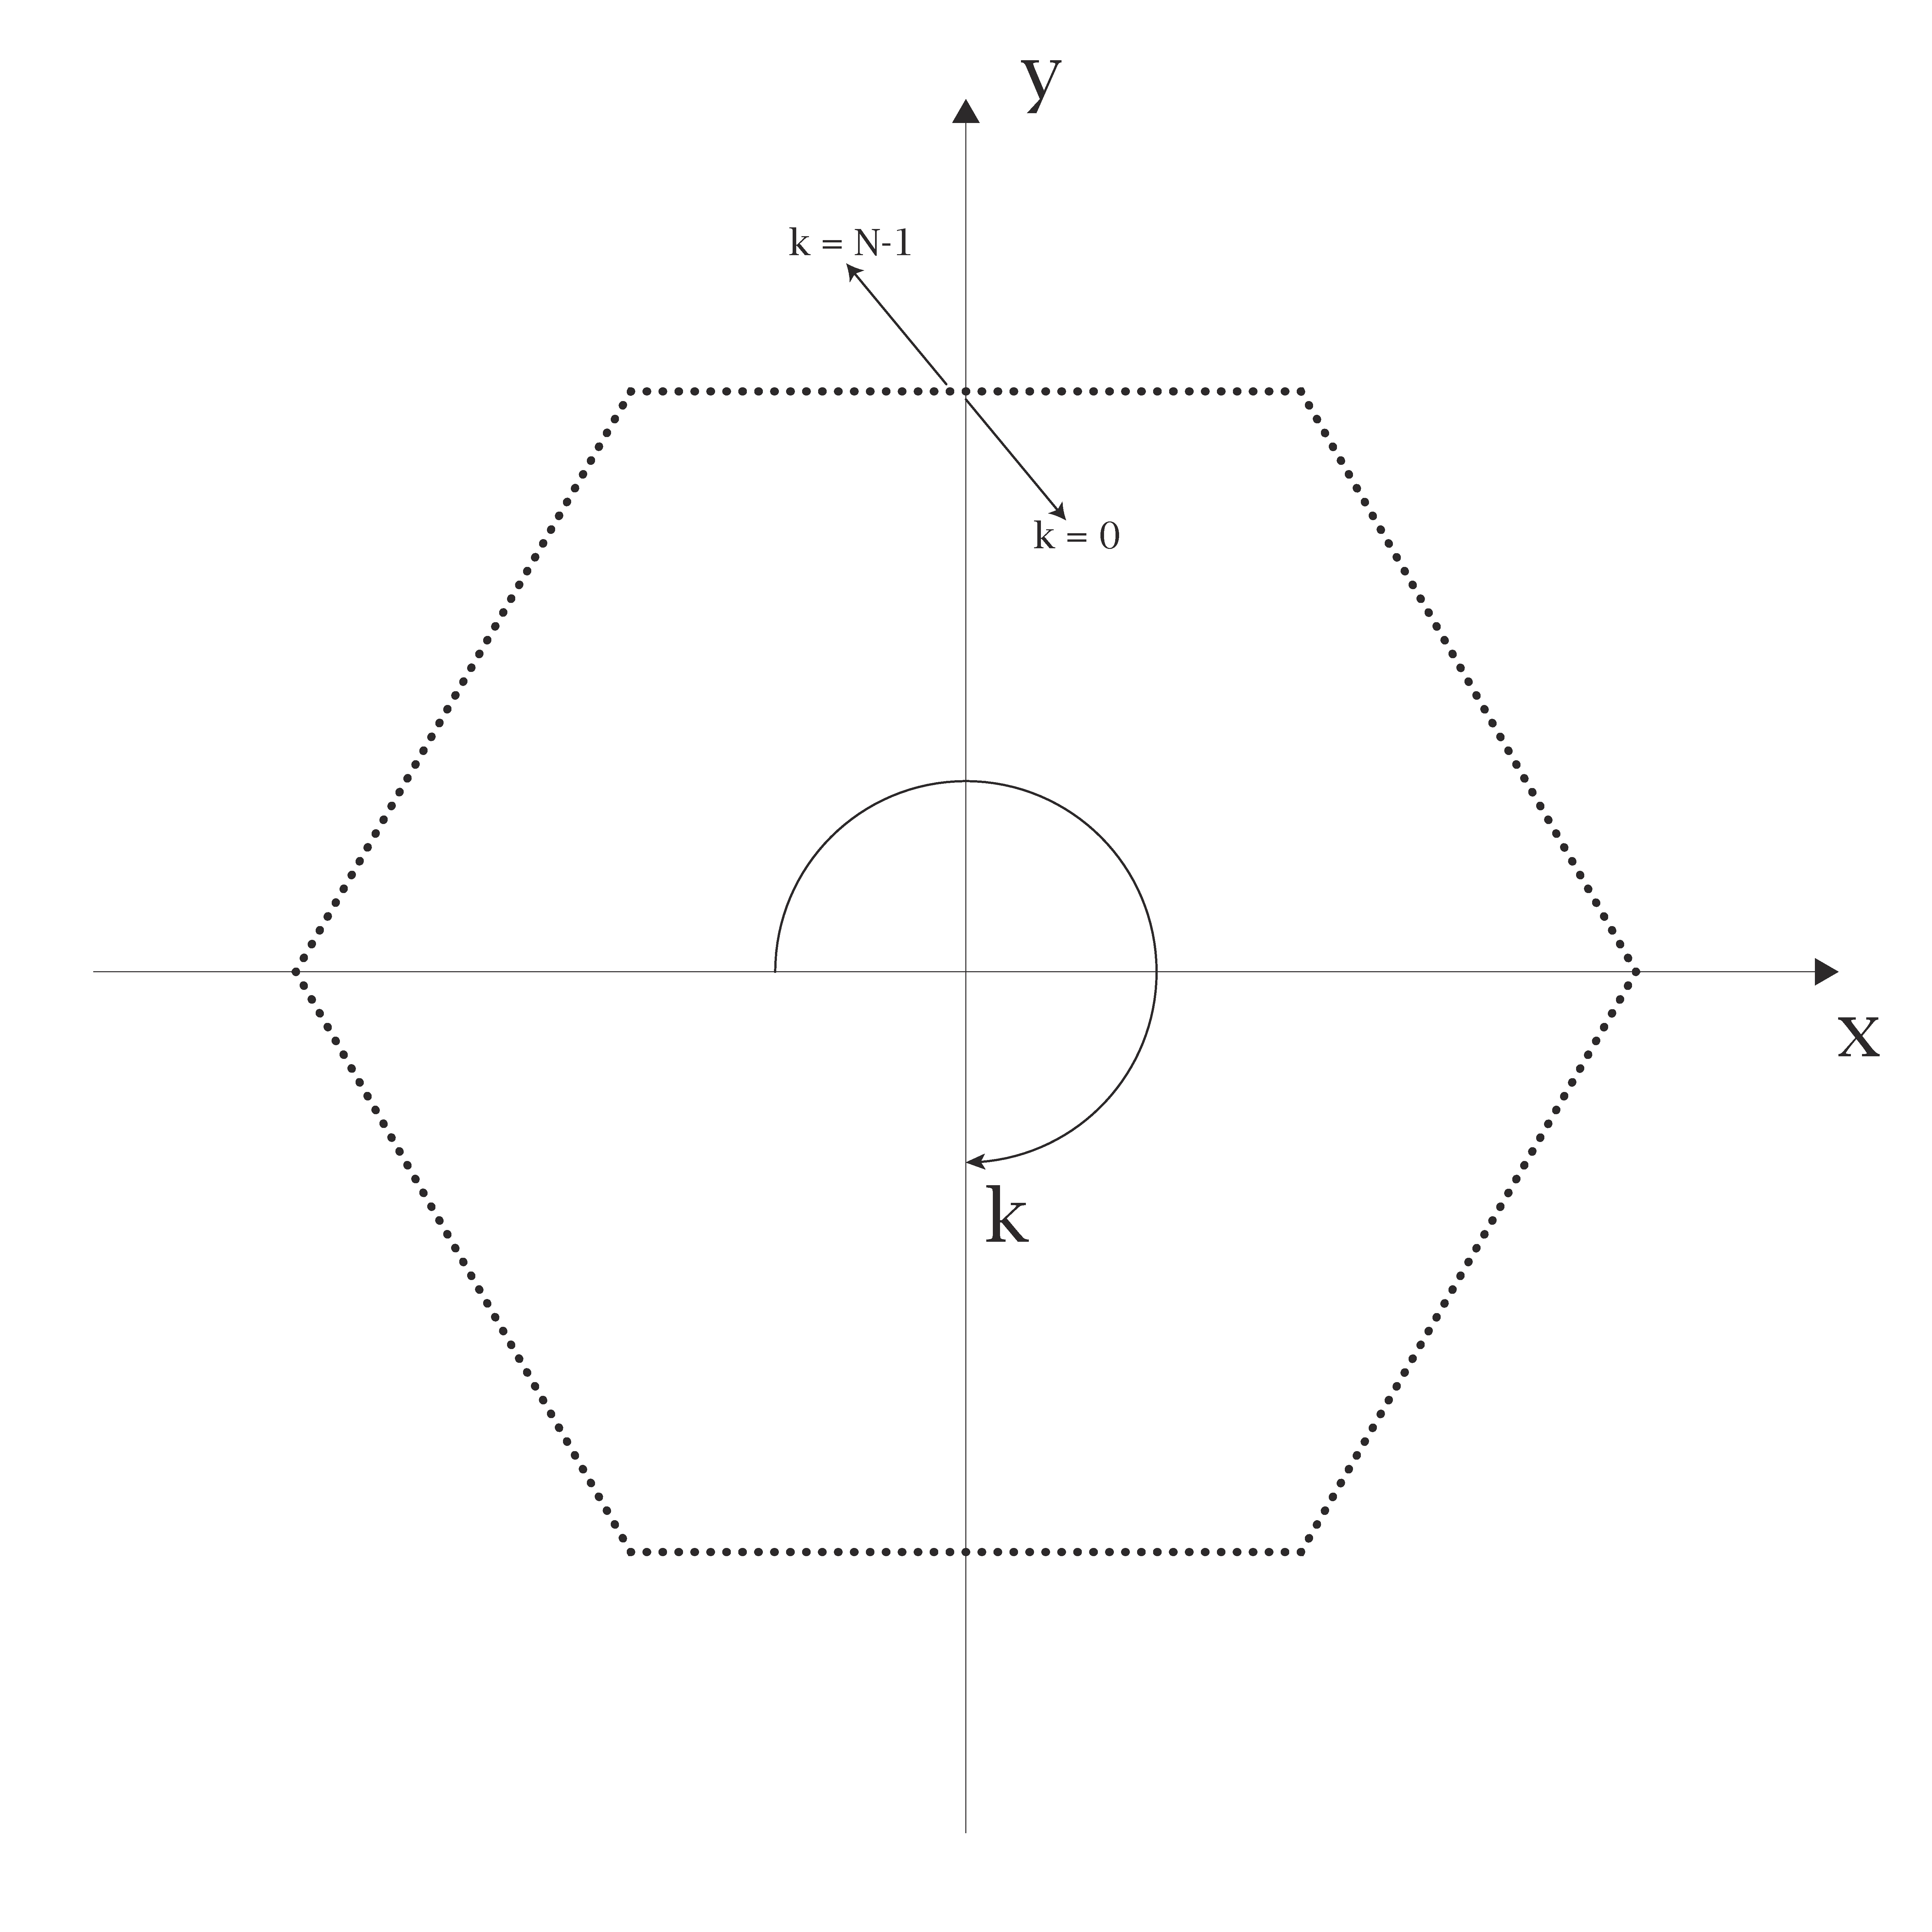
\includegraphics[width=0.7\textwidth]{imagenes/marco_teorico/Descriptores_Fourier/Poligono_ejesXY_k_figura.pdf}	
		\caption{}
		\label{fig:fourier_poligono_trazo_discontinuo}
	\end{subfigure}	
	\caption{Descriptores de Fourier}
	\label{fig:fourier_esquema}
\end{figure}

Este nuevo contorno está representado por $N$ puntos, de tal forma que cada punto puede definirse de la forma $ (x_{k},\:y_{k}),\:con\:k = 0, 1, 2, ..., N-1 $ y el contorno, a su vez, como la señal $f_{k} = (x_{k},\:y_{k})$.

Si $f_{k}$ es transformada al dominio complejo de la forma $f_{k} = x_{k} + iy_{k}$, es posible aplicar la transformada discreta de Fourier a $f_{k}$ para obtener los $N$ armónicos de la señal (descriptores de Fourier): 

\begin{equation}
	F_{m} = \sum_{k=0}^{N-1} f_{k}\cdot e^{-\dfrac{2\pi i}{N}mk},\qquad m = 0, 1, 2, ..., N-1
	\label{eqn:dft}
\end{equation}

La ecuación \ref{eqn:dft} (transformada discreta de Fourier), proporciona la serie de valores $ F_{0}, F_{1}, F_{2}, ..., F_{N-1} $, a partir de los cuales se obtienen los descriptores de Fourier (valores absolutos) $\lvert F_{0}, F_{1}, F_{2}, ..., F_{N-1} \rvert$.

En función de la resolución de la imagen original y su definición, el número de puntos del contorno $N$ variará, obteniéndose una cantidad diferente para cada caso. Por ello, el número de descriptores de Fourier obtenibles de cada imagen no será el mismo. Es por esto que, generalmente, de los $N$ descriptores obtenidos para cada imagen, se escogen solo $n\:|\:0\leq n\leq N$.

\begin{figure}[H]
	\centering
	\captionsetup{justification=centering}
	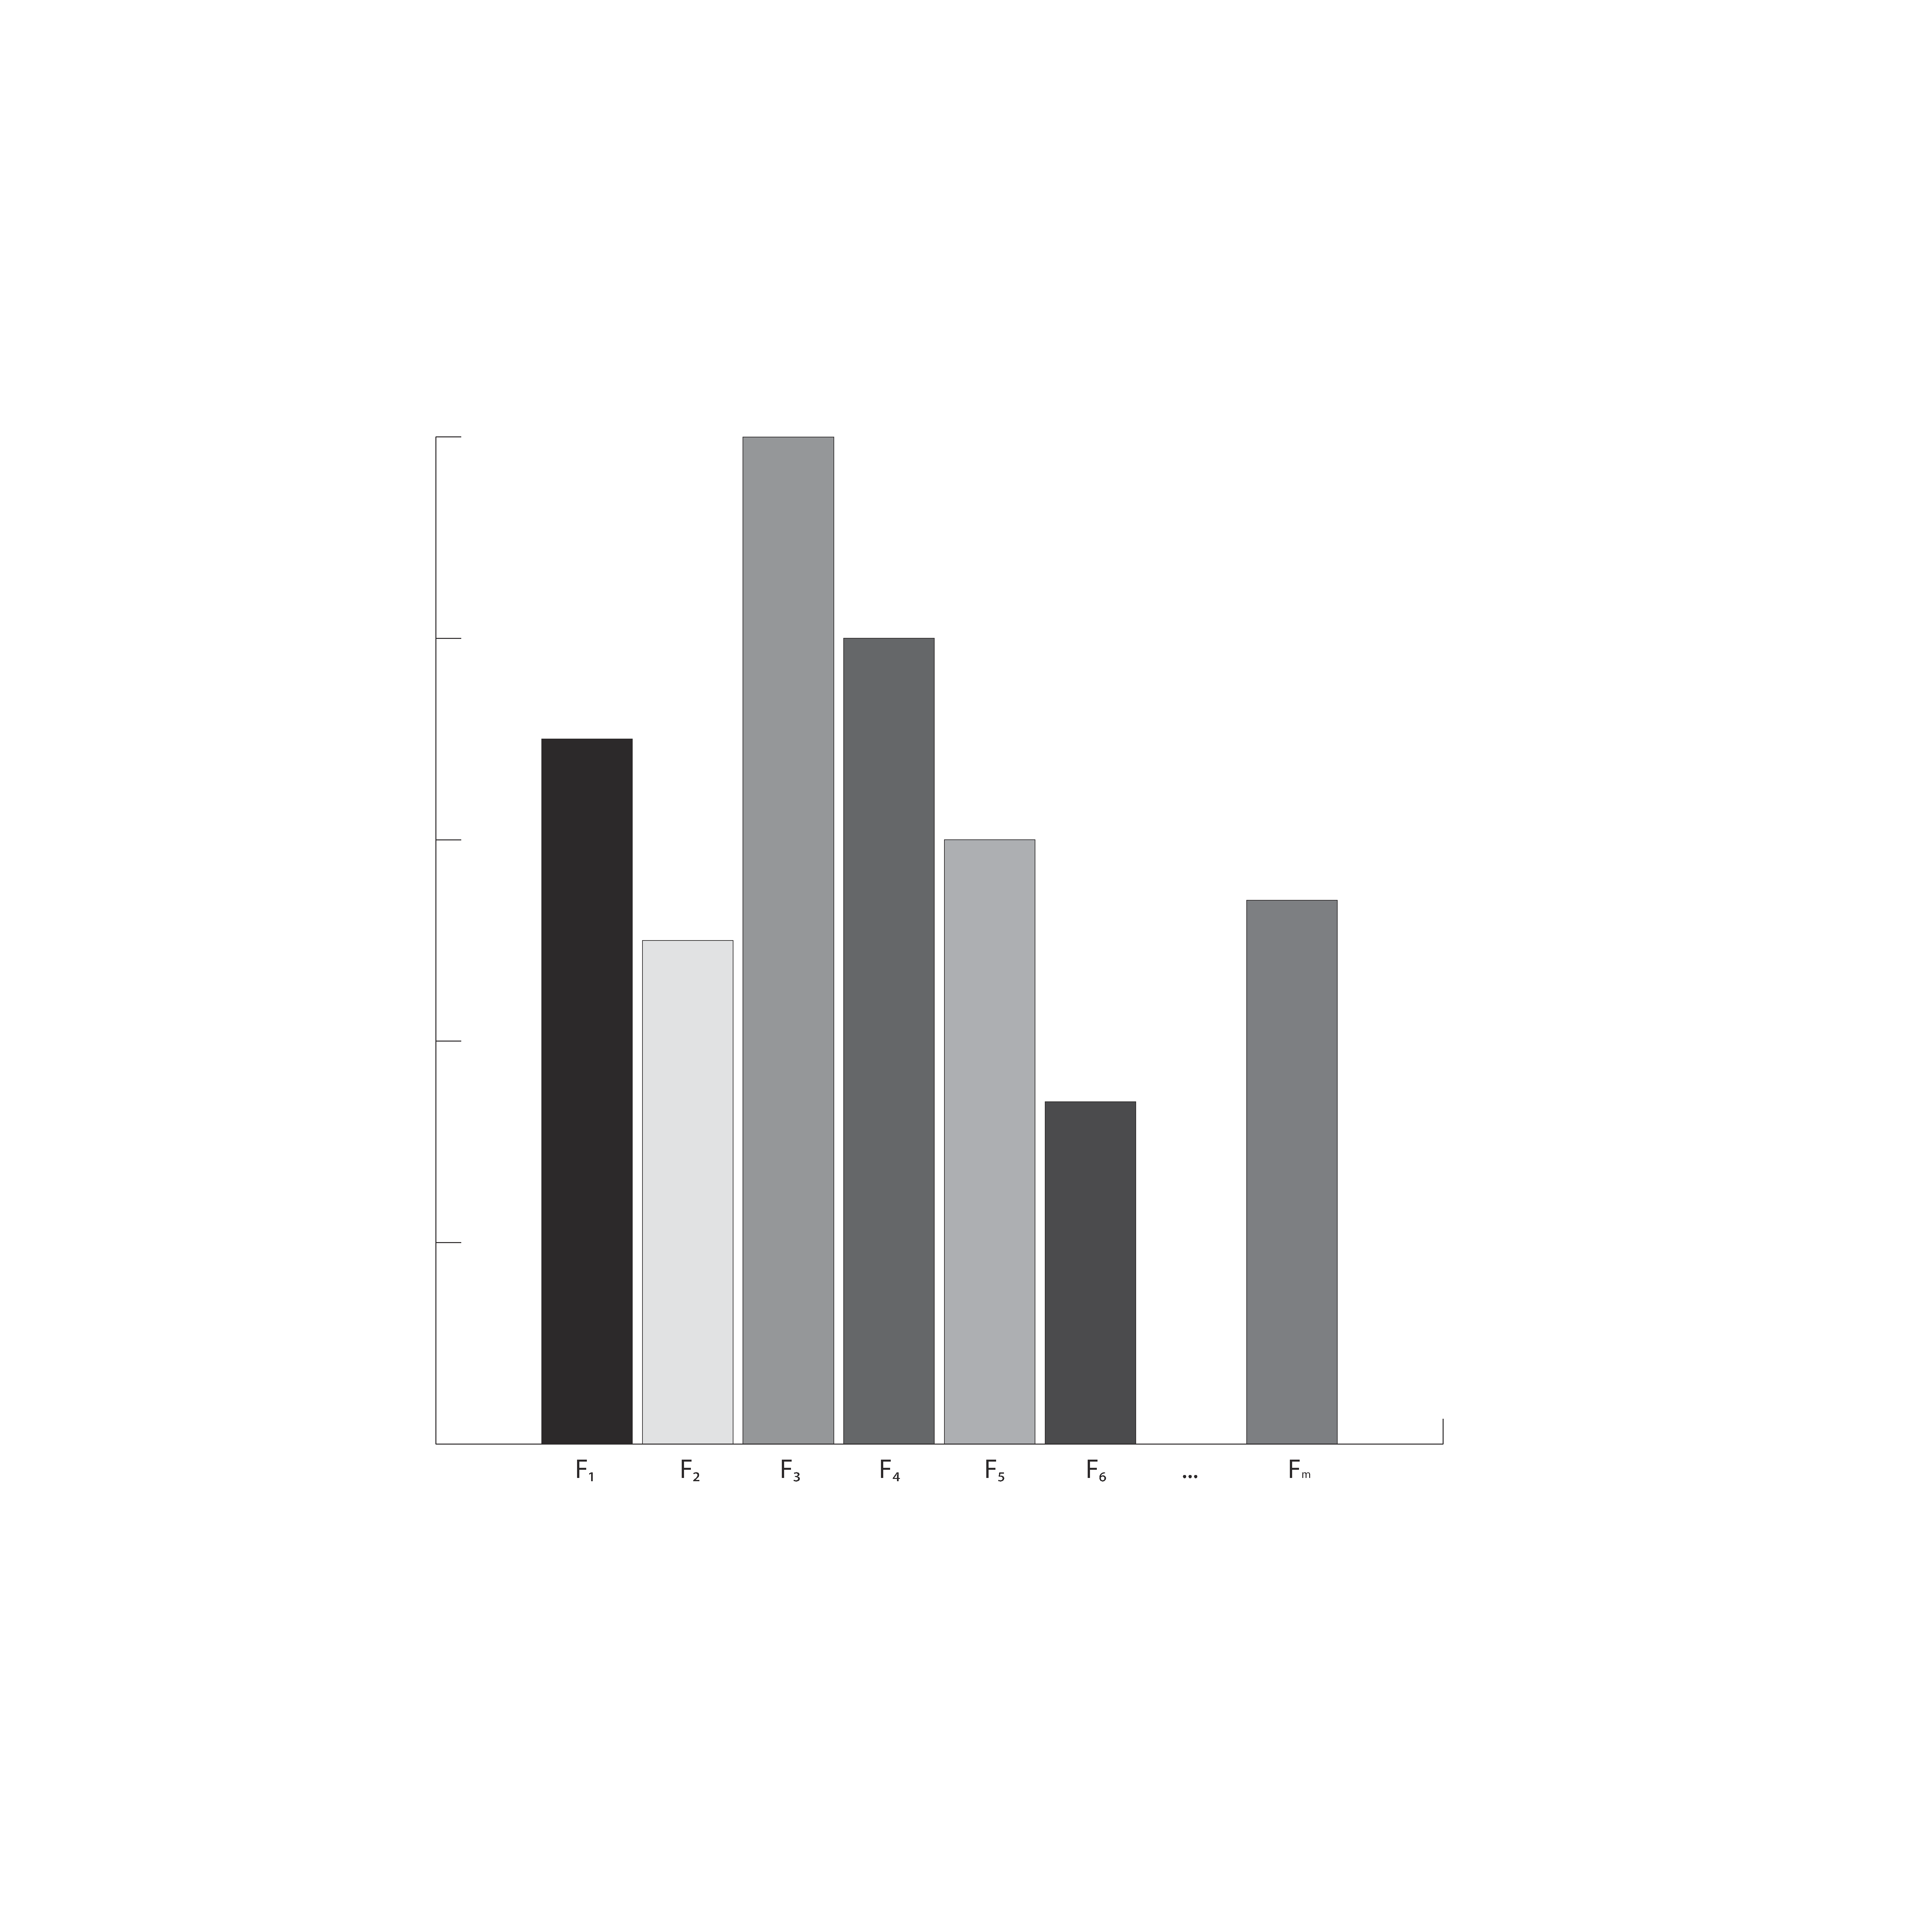
\includegraphics[width=\textwidth]{imagenes/marco_teorico/Descriptores_Fourier/Histograma_ejemplo_generico.pdf}
	\caption{}	
	\label{fig:fourier_histograma_generico_ejemplo}
\end{figure}

%% -----------------------------------------------------------------------%%

\section{Selección de características}

Una vez se han aplicado los métodos propuestos en la sección \ref{section:Extracción de catacterísticas}, es necesario realizar un análisis del poder clasificatorio de las características extraídas.

Para este trabajo, se han utilizado los siguientes métodos:
\begin{itemize}
	\item ANOVA
	\item SFS
\end{itemize}

\subsection{ANOVA}

\mynote{ANOVA es un conjunto de métodos estadísticos, entre los cuales está el F-Test, que es el que se usa aquí, principalmente.}

\mynote{Casi toda la información está sacada de \cite{frost_2020}.}

Conocido como Análisis de la Varianza (del inglés, \textit{ANalysis Of VAriance}).

Dado un ejemplo como una distribución de datos de dos clases (véase figura \ref{ANOVA:distribucion_ejemplo}), se disponen de dos características de clasificación: $(x,y)$.

\begin{figure}[h]
	\centering
	\captionsetup{justification=centering}
	\includegraphics[scale = 0.5]{imagenes/marco_teorico/ANOVA/ejemplo_distribuciones.png}
	\caption{Distribuciones para un caso ejemplo de ANOVA}
	\label{ANOVA:distribucion_ejemplo}
\end{figure}

La característica $x$ es mucho mejor que la $y$ a simple vista pues, comparando las distribuciones de ambas, para $x$ se obtienen dos distribuciones claramente separadas por completo, mientras que para la característica $y$ las distribuciones se solapan.

También se puede comprobar que la distribución para la característica $x$ presenta una menor varianza (son más compactas) que con $y$.

Por tanto, para este ejemplo se puede definir la condición \ref{eqn:anova_1} como un parámetro de discriminación de características. Cuanto mayor sea para una característica, mejor será su poder de clasificación.

\begin{equation}
	F = \dfrac{Distancia\:entre\:clases}{Compacidad\:de\:clases}
	\label{eqn:anova_1}
\end{equation}

Matemáticamente, la fórmula \ref{eqn:anova_1} puede expresarse de la siguiente forma siguiendo el método ANOVA:

\begin{itemize}
	\item El numerador (distancia entre clases) es definible con:
	\begin{equation}
		n_{azul}(\overline{x_{azul}}-\overline{x})^{2} + n_{rojo}(\overline{x_{rojo}}-\overline{x})^{2}
	\end{equation}
	\item El denominador (compacidad de clases), que no es sino la varianza de clases, puede expresarse como:
	\begin{equation}
		\left(\dfrac{1}{(n_{azul}-1)+(n_{roja}-1)}\right)\left(\sum_{i=1}^{n_{azul}}\left(x_{i}-\overline{x_{azul}}\right)^{2}+\sum_{i=1}^{n_{roja}}\left(x_{i}-\overline{x_{roja}}\right)^{2}\right)
	\end{equation}
\end{itemize}

De tal forma, la ecuación \ref{eqn:anova_1} queda como:

\begin{equation}
	F = \dfrac{n_{azul}(\overline{x_{azul}}-\overline{x})^{2} + n_{rojo}(\overline{x_{rojo}}-\overline{x})^{2}}{\left(\dfrac{1}{(n_{azul}-1)+(n_{roja}-1)}\right)\left(\sum_{i=1}^{n_{azul}}\left(x_{i}-\overline{x_{azul}}\right)^{2}+\sum_{i=1}^{n_{roja}}\left(x_{i}-\overline{x_{roja}}\right)^{2}\right)}
	\label{eqn:ANOVA}
\end{equation}

La ecuación \ref{eqn:ANOVA} da un parámetro para una variable (en este caso $x$). En un problema con $k$ características, se obtendrían $k$ valores de $F$, es decir, una $F$ para cada variable.

Utilizando las $k$ características extraídas con los métodos propuestos en \ref{section:Extracción de catacterísticas}, ANOVA proporcionaría $F_{k}$ valores, de entre los cuales se seleccionarían los $N$ con mayor valor $F$. La ecuación \ref{eqn:ANOVA_F} define el valor de F para un caso con $j = 1,\:2,\:3,\:...,\:N$ clases. 

\begin{equation}
	F = \dfrac{\sum_{j=1}^{N} n_{j}\left(\overline{x_{i}}-\overline{x}\right)^{2}}{\left(\dfrac{1}{\sum_{j=1}^{N}(n_{j}-1)}\right) \left(\sum_{j=1}^{N}\left(\sum_{i=1}^{n_{j}}(x_{i}-\overline{x_{j}})^{2}\right)\right)}
	\label{eqn:ANOVA_F}
\end{equation}

\mynote{Este método solo da información sobre lo bien que UNA variable discrimina, pero no dice como de bien lo harían varias juntas.}

\subsection{SFS}

Los algoritmos SFS (del inglés \textit{Sequential Feature Selector} son un conjunto de técnicas de selección de caracteríticas (algoritmos voraces) usados para reducir un espacio incial n-dimensional de características a otro k-dimensional donde $k\leq d$.

Si se tiene el siguiente conjunto n-dimensional $Y = \{y_{1},y_{2},y_{3},...,y_{n}\}$ de características de entrada, utilizando un estimador determinado (SVM, Knn, SDG, etc.) y una métrica de rendimiento determinada, el algoritmo SFS busca obtener un conjunto de salida $X_{k} = \{x_{j} | j = 1,2,...,d;\: x_{j}\epsilon Y\},\: con \:k = (0,1,2,...,n)$ tal que $X_{k}$ esté formado por las $k$ características que maximicen la métrica.

Existen dos formas de realizar este proceso: hacia adelante (\textit{Forward}) y hacia detrás (\textit{Backwards}).

\begin{itemize}
	\item Sequential Forward Selection: se comienza con un conjunto vacío $X_{0} = \emptyset / k = 0$. En cada iteración se aumenta el número de características hasta encontrar la combinación que de el mejor resultado (según la métrica a resolver).
	\item Sequential Backward Selection: se comienza con el conjunto inicial $Y$. En cada iteración se disminuye el número de características hasta encontrar la combinación que de el mejor resultado (según la métrica a resolver).
\end{itemize}

Es posible no llegar al mismo resultado empleando sentidos contrarios y tampoco obtener el mismo resultado, en varias iteraciones, utilizando el mismo método.

\mynote{En \textit{Sklearn} la métrica para su modelo SFS es una evaluación de validación cruzada con un estimador definido en la llamada al método SFS.}

\newpage
\section{Métodos de evalución}

Antes de entrar en la sección de modelos de clasificación, es necesario definir las métricas propuestas utilizadas para analizar los resultados de los clasificadores.

En una primera instancia, es necesario presentar la \nameref{tab:matriz_confusion}.

\subsection{Matriz de confusión}

\begin{table}[h]
	\centering
	\caption{Matriz de confusión binaria}
	\label{tab:matriz_confusion}
	\begin{tabular}{cc|cc|}
		\cline{3-4}
		&  & \multicolumn{2}{c|}{Valor real} \\ \cline{3-4} 
		&  & \multicolumn{1}{c|}{1}    & 0   \\ \hline
		\multicolumn{1}{|c|}{Valor}    & 1 & \multicolumn{1}{c|}{True Positive (TP)}  & False Positive (FP) \\ \cline{2-4} 
		\multicolumn{1}{|c|}{predicho} & 0 & \multicolumn{1}{c|}{False Negative (FN)} & True Negative (TN)  \\ \hline
	\end{tabular}
\end{table}

La matriz de confusión es una herramienta muy utilizada para representar y ver de forma sencilla los resultados de una clasificación. En el caso de la tabla \ref{tab:matriz_confusion}, se representa una matriz de confusión para un caso de clasificación binaria, sin embargo puede utilizarse para casos multiclases.

A partir de la matriz de confusión binaria se obtienen las métricas de rendimiento de evaluación de un clasificador: exactitud, precisión, exhaustividad, f1, etc.

\begin{equation}
	\mbox{Exactitud (ACC)} = \dfrac{TP+TN}{TP+TN+FP+FN}
	\label{eqn:accuracy}
\end{equation}

\begin{equation}
	\mbox{Exhaustividad (TPR)} = \dfrac{TP}{P} = \dfrac{TP}{TP+FN}
	\label{eqn:exhaustividad}
\end{equation}

\begin{equation}
	\mbox{Precision} = \dfrac{TP}{TP+FP}
	\label{eqn:precision}
\end{equation}

\begin{equation}
	F_{\beta} = \left(1+\beta^{2}\right) \dfrac{2\cdot \mbox{Precision}\cdot \mbox{Exhaustividad}}{\mbox{Precision}+\mbox{Exhaustividad}}
	\label{eqn:fbeta_score}
\end{equation}

\begin{itemize}
	\item Exactitud: (en inglés \textit{accuracy}) (ecuación \ref{eqn:accuracy}) es una medida de la proporción de predicciones correctas (tanto TP como TN) del total de casos a predecir.
	\item Precisión: (ecuación \ref{eqn:precision}) medida del porcentaje de valores positivos acertados (TP) de entre todos los valores positivos predichos (TP+FP). La precisión muestra la robustez del clasificador para acertar en los resultados positivos. Sin embargo, no tiene en cuenta como de bueno es acertando las clases negativas.
	\item Exhaustividad: (en inglés \textit{recall}) (ecuación \ref{eqn:exhaustividad}) medida del porcentaje de las muestras positivas predichas correctamente como positivas (TP) entre el numero total de muestras positivas reales (TP+FN). La exhaustividad es una medida de la capacidad del clasificador para detectar muestras positivas. A mayor \textit{recall}, mas muestras positivas (correctas e incorrectas) detecta. Sin embargo, es una métrica que no tiene para nada en cuenta la clasificación de muestras negativas reales (FP y TN).
	\item F-score: es una media armónica de la exhaustividad y la precisión. En función del parámetro $\beta$, se le da peso a la exhaustividad. A mayor valor de $\beta$, mas importanto el \textit{recall}. Es muy común utilizar la métrica para $\beta=1$, es decir, \textit{F1-score}, misma valoración tanto a la precisión como a la exhaustividad. Sin embargo, la métrica $F_{1}$ no considera los negativos verdaderos (TN) (ni \ref{eqn:exhaustividad}, ni \ref{eqn:precision} usan TN en sus cálculos) y para problemas con clases desbalanceadas es erróneo usar esta métrica, prefiriendo el uso del coeficiente de 	Kappa\cite{https://doi.org/10.48550/arxiv.2010.16061}.
\end{itemize}

\paragraph{Exactitud con problemas desbalanceados} \label{par:exactitud_mala} Si se supone un ejemplo donde se tiene un dataset de 10000 muestras de personas enfermas con gripe o coronavirus, del cual 9990 muestras son de personas con gripe, el clasificador podría asignar ciegamente a cada nueva muestra la condición de gripe y sería exacto en un $99.9\%$ de las veces. Lo que implica que la métrica de exactitud no es correcta para casos desbalanceados.

\subsubsection{Matriz de confusión para problemas multiclases}

Para problemas con más de 2 clases, la matriz de confusión \ref{tab:matriz_confusion} se convierte en \ref{tab:matriz_confusion_multiclase}, donde se representa el número de muestras de una clase que han sido identificadas como de otra clase o de si misma. Además de ser simétrica respecto de la diagonal.

\begin{table}[H]
	\centering
	\caption{Matriz de confusión multiclase}
	\label{tab:matriz_confusion_multiclase}
	\begin{tabular}{|c|c|c|c|c|}
		\hline
		Clase & 1 & 2 & ... & N \\ \hline
		1     & X &   &     &   \\ \hline
		2     &   & X &     &   \\ \hline
		...   &   &   & X   &   \\ \hline
		N     &   &   &     & X \\ \hline
	\end{tabular}
\end{table}

Para este caso, las variables la matriz de confusión binaria cambian de definición. Las predicciones correctas de cada clase con si misma (marcadas con X en la tabla \ref{tab:matriz_confusion_multiclase}) corresponden a los verdaderos positivos (TP); el sumatorio de los valores de cada fila, excepto el valor X, corresponde a los falsos positivos (FP); para una clase $N$, el sumatorio de todas las predicciones erróneas de las demás clases que predijeron pertenecer a la clase $N$ es el falso negativo (FN) de la $N$; y para una clase $N_{i}$ el sumatorio de los verdaderos positivos (TP) del resto de clases es TN (verdadero negativo) para la clase $N_{i}$. (Véase \nameref{par:convertir_matriz_binario_multiclase}).

Las métricas de exactitud, precisión, exhaustividad y $F_{1}$, para este caso, son aplicables en cuanto a cada clase se refiere. Para $N$ clases se obtienen $N$ métricas, sin embargo, es deseable obtener un solo valor, de cada métrica, que represente a todas las clases. Para ello, es necesario hacer un promediado 'micro', 'macro' o ponderado.

\subsubsection{Promediado 'micro', 'macro' y ponderado.}

\begin{table}
	\centering
	\begin{tabular}{|c|c|c|c|} 
		\hline
		Clase & F1  & Precisión & Recall  \\ 
		\hline
		1     & $F_{1_1}$ & $P_{1}$        & $P_{1}$      \\ 
		\hline
		2     & $F_{1_2}$ & $P_{2}$        & $P_{2}$      \\ 
		\hline
		3     & $F_{1_3}$ & $P_{3}$        & $P_{3}$      \\
		\hline
	\end{tabular}
\end{table}

\begin{itemize}
	\item Macro: consiste en obtener la media aritmética entre clases. Da un mismo peso a todas las clases.
		\begin{equation}
			P = \dfrac{P_{i}+P_{i+1}+P_{i+2}+\mbox{...}+P_{N}}{N}
		\end{equation}
	\item Micro: consiste en aplicar la fórmula de cada métrica con el sumatorio total de variables de cada clase. 
		\begin{equation}
			P = \dfrac{\sum_{i=1}^{N} TP_{i}}{\sum_{i=1}^{N} \left(TP_{i}+FP_{i}\right)}
		\end{equation}
	\item Ponderado: consiste en aplicar la frecuencia de cada clase en el dataset total al sumatorio de métricas.
		\begin{equation}
			P = \sum_{i=1}^{N} P_{i}f_{i}; \mbox{ donde } f_{i} = \dfrac{N_{i}}{N}
		\end{equation}
\end{itemize}

Tómese por ejemplo un caso de clasificación desbalanceada de tres clases según la matriz de confusión \ref{tab:ejemplo_promedios} y las métricas de cada clase \ref{tab:ejemplo_promedios_metricas}.

\begin{table}[H]
	\centering
	\captionsetup{justification=centering}
	\begin{tabular}{|c|c|c|c|}
		\hline
		Clase & 0    & 1    & 2   \\ \hline
		0     & 5331 & 1921 & 748 \\ \hline
		1     & 1014 & 357  & 129 \\ \hline
		2     & 344  & 122  & 34  \\ \hline
	\end{tabular}
	\caption{Ejemplo matriz de confusión para métricas ponderadas}
	\label{tab:ejemplo_promedios}
\end{table} 

\begin{table}[H]
	\centering
	\captionsetup{justification=centering}
	\begin{tabular}{|c|c|c|c|c|}
		\hline
		Clase & Precisión & Recall & F1   & Nº de muestras \\ \hline
		0     & 0.8       & 0.67   & 0.73 & 8000           \\ \hline
		1     & 0.15      & 0.24   & 0.18 & 1500           \\ \hline
		2     & 0.04      & 0.07   & 0.05 & 500            \\ \hline
	\end{tabular}
	\caption{Ejemplo métricas para caso desbalanceado}
	\label{tab:ejemplo_promedios_metricas}
\end{table}

La tabla \ref{tab:ejemplo_promedios_metricas2} muestra las métricas promedio:

\begin{table}[H]
	\centering
	\captionsetup{justification=centering}
	\begin{tabular}{|c|c|c|c|c|}
		\hline
		Clase     & Precisión & Recall & F1     & Nº de muestras \\ \hline
		Micro     & 0.5722    & 0.4856 & 0.4433 & 8000           \\ \hline
		Macro     & 0.3276    & 0.3241 & 0.3190 & 1500           \\ \hline
		Ponderada & 0.6617    & 0.8322 & 0.611  & 500            \\ \hline
	\end{tabular}
	\caption{Ejemplo métricas promedio}
	\label{tab:ejemplo_promedios_metricas2}
\end{table}

Para cualquiera de las tres métricas, $\mbox{Macro} < \mbox{Micro} < \mbox{Ponderada}$. Tomando como referencia la tabla \ref{tab:ejemplo_promedios_metricas}, para la precisión (por ejemplo), la clase cero tiene un valor muy elevado respecto a las otras dos, incluso se puede decir que el clasificador es nefasto con las clases dos y tres. Cuando se calcula la precisión macro, se realiza un simple media entre las precisiones, dándole el mismo peso ó importancia a cada clase, por tanto, los valores reducidos de las clases dos y tres contribuyen a bajar mucho el valor de la precisión total del problema, aún cuando para la clase cero es muy elevada. Para el caso ponderado, como a cada precisión se le multiplica por su frecuencia en el dataset, la clase cero contribuye a aumentar mucho el valor pues, tiene 8000 muestras ella sola frente a las 2000 de las clases una y dos. La precisión micro obtiene un valor intermedio ya que tiene en cuenta los falsos positivos de cada clase, aumentando la influencia de la clase más frecuente ya que sus falsos positivos serán mayores al tener más muestras.

Por tanto, en general, para casos desbalanceados, si se considera a cada clase igual de importante que las demás, es conveniente utilizar un promedio macro. Si, por el contrario, es la clase más frecuente la más importante, el promedio ponderado es el preferible. Si se desea obtener un resultado que favorezca a la muestra más frecuente sin considerarla la más importante, un promedio micro es considerable.

No siempre ocurre que la micro es mayor que la macro pues, depende de los datos. Si la clase más frecuente tiene la métrica más pequeña con las demás siendo muy elevadas, es probable que la micro resulte de menor magnitud que la macro (a diferencia del ejemplo presentado), ya que la micro favorece a la clase más frecuente, sin llegar al punto de la ponderación.

Ya que, al final, depende del caso, es imprescindible contar con algo más de información (matriz de confusión, por ejemplo) para poder interpretar correctamente los datos.

\paragraph{Conversión de problema multiclase a binario}\label{par:convertir_matriz_binario_multiclase} Es posible convertir un problema de clasificación multiclase a un conjunto de problemas binarios utilizando los métodos \nameref{par:OVR} o \nameref{par:OVO}.

\subsection{Curva ROC} \label{subsection:ROC_curva}

Lo habitual, además de deseable, a la hora de obtener los valores predichos de un clasificador, es hacerlo en forma de estimaciones probabilísticas en el rango $[0,\:1]$. De tal forma que, cuando se obtenga un valor, se puede comprobar con qué nivel de confianza el clasificador asigna a qué clase la muestra a predecir.

Muchas librerías de algoritmos supervisados devuelven los resultados, por defecto, como valores enteros $0$ o $1$, aplicando un umbral de clasificación de $0.5$. En el caso de obtener $0.5000001$ para la clase positiva y $0.4999999$ para la negativa, el clasificador asignaría automáticamente la muestra a la clase positiva, obviando el hecho de que realmente no existe un nivel de confianza suficiente para clasificar la muestra de tal forma.

Al obtenerse probabilidades y no valores discretos, para asignar clases, es necesario establecer un umbral de clasificación por el cual si $p(n) \geq umbral \rightarrow n = 1$. Por tanto, es conveniente encontrar un valor para el umbral de clasificación que haga que el clasificador funcione lo mejor posible.

Para cada valor de umbral se obtiene una matriz de confusión diferente, así como sus pertinentes métricas. Puede que exista un valor de umbral en el que el clasificador, para la base de datos dada, sea idóneo o puede que no existe ningún valor de umbral que haga que el clasificador discrimine correctamente. Sin embargo, es posible que, independientemente del umbral, el clasificador obtenga buenos resultados.

Para poder analizar estos casos, se recurre a la curva ROC (del inglés \textit{Receiver operating characteristic}).

La curva ROC es un gráfico utilizado para determinar la habilidad discriminante de un clasificador binario según su umbral de clasificación es variado.

Este gráfico se basa en el espacio ROC, que es básicamente la representación de la tasa de verdaderos positivos (o exhaustividad) (\ref{eqn:exhaustividad}) frente a la tasa de falsos positivos (\ref{eqn:fpr}).

\mynote{Exhaustividad: cantidad de valores reales positivos predichos como positivos.}

\begin{equation}
	Tasa\: de\: falsos\: positivos\:(FPR) = \dfrac{FP}{N} = \dfrac{FP}{FP+TN}
	\label{eqn:fpr}
\end{equation}

\begin{figure}[h]
	\centering
	\captionsetup{justification=centering}
	\includegraphics[width=0.5\textheight]{imagenes/marco_teorico/ROC/ROC_wiki.png}	
	\caption{Sacado de wikipedia (EDITAR)}
	\label{fig:roc_curva}
\end{figure}

La línea de puntos roja representa un clasificador puramente aleatorio que asigna un $0.5$ de probabilidades de pertenecer a la clase positiva a cada muestra.

Para valores de umbral en el rango $[0,\:1]$, se obtienen los valores de \ref{eqn:exhaustividad} y \ref{eqn:fpr}, y se representa el punto correspondiente en el gráfico. De tal forma, se obtiene una curva escalonada que representa la calidad del clasificador.

El caso idóneo es aquel en el que la curva del clasificador es un escalón unidad, es decir, aquel clasificador que, para cualquier valor de umbral, se obtiene un 100\% de exhaustividad. Numéricamente, este tipo de curva corresponde a una curva con una área bajo la curva de la unidad.

El peor caso es el clasificador cuya curva sea la inversa al escalón unidad pues, se obtiene un 0\% de exhaustividad para cualquier umbral, es decir, aquella curva con una área bajo la curva nula.

Por tanto, se define el parámetro \textbf{AUC}, del inglés \textit{Area Under the Curve}, que determina la calidad discriminante del clasificador. Cuanto mayor sea el valor de AUC, mejor el clasificador.

Sin embargo, la curva ROC no es correcta para casos desbalanceados ya que no representa correctamente los resultados, siendo necesario sustituirla por una curva de precisión-exhaustividad \cite{10.1371/journal.pone.0118432}. 

\paragraph{Clasificación multiclase} La curva ROC y sus derivadas sólo son utilizables para problemas binarios. Para casos con más de dos clases, se requiere una \nameref{par:OVR}, obteniendo tantas curvas ROC como clases, así como un valor AUC para cada clase, que representaría la calidad del clasificador de discriminar esa clase respecto a las demás; o \nameref{par:OVO}, obteniendo $\dfrac{N(N-1)}{2}$ curvas ROC y valores AUC.

\subsection{Validación cruzada}

Todo proceso de clasificación necesita de dos conjuntos de datos para entrenamiento y validación de resultados.

Lo más simple es dividir el dataset de partida en dos particiones: entrenamiento y validación.

\begin{figure}[h]
	\centering
	\captionsetup{justification=centering}
	\includegraphics[width=\textwidth]{imagenes/marco_teorico/CV/train_test_split.pdf}
	\label{fig:CV_train_test_split}
	\caption{División de dataset en entrenamiento y validación}
\end{figure}

Sin embargo, cabe la posibilidad de que al dividir el dataset, los datos de la partición de entrenamiento sean diferentes a la de validación. Es decir, puede que los datos de entrenamiento no sean suficientemente generalistas (atípicos) y al validar el modelo con los datos de validación, se obtengan resultados muy pobres. Para evitar esto se recurre a la validación cruzada.

Del inglés \textit{Cross-Validation}, la validación cruzada es un método de análisis de resultados en modelos de clasificación que garantiza la independencia de los resultados frente a la división de datos de entrenamiento y validación.

El dataset inicial es dividido en $N$ particiones (además, es de buenas prácticas mezclar los datos entre particiones) y cada partición es dividida en $N$ partes. $N-1$ partes de cada partición son empleadas para entrenar el modelo y la parte restante para validación. Este proceso se repite para todas las particiones, obteniendo $N$ resultados.

La figura \ref{fig:CV_cv4} representa una validación cruzada de cuatro particiones.

\begin{figure}[h]
	\centering
	\captionsetup{justification=centering}
	\includegraphics[width=\textwidth]{imagenes/marco_teorico/CV/cv_4.pdf}
	\caption{Validación cruzada de 4 particiones}
	\label{fig:CV_cv4}
\end{figure}

Con los $N$ resultados se realizan análisis estadísticos (principalmente media y desviación típica) para obtener métricas independientes del punto de división de la base de datos.

%\subsubsection{Métricas de rendimiento}
%
%A partir de la matriz de confusión se obtienen las llamadas métricas de rendimiento. Estos parámetros son utilizados en sistemas de clasificación, reconocimiento de patrones, etc, para analizar los resultados de dichos modelos.
%
%%\begin{itemize}
%%	\item Sensitividad, exhaustividad, tasa de positivos verdaderos: cantidad de valores reales positivos predichos como positivos.
%%		\begin{equation}
%%			Exhaustividad = \dfrac{TP}{P} = \dfrac{TP}{TP+FN}
%%			\label{eqn:exhaustividad}
%%		\end{equation}
%%	\item Exactitud: cantidad de predicciones que el modelo acertó.
%%		\begin{equation}
%%			Exactitud = \dfrac{TP+TN}{P+N} = \dfrac{TP+TN}{TP+TN+FP+FN}
%%			\label{eqn:exactitud}
%%		\end{equation}
%%	\item Precisión: cantidad de predicciones positivas acertadas correctamente.
%%		\begin{equation}
%%			Precision = \dfrac{TP}{TP+FP}
%%			\label{eqn:precision}
%%		\end{equation}
%%\end{itemize}
%
%Como se presenta en \cite{10.1371/journal.pone.0118432}, no todas las métricas de rendimiento son correctas para cualquier caso de clasificación, viéndose afectadas para casos desbalanceados.
%
%\mynote{Un caso desbalacenado de clasificación, binario o multiclase, es aquel donde la frecuencia de muestras de cada clase no es similar al del resto de clases. Es decir, para un caso binario, lo más común es tener muchas más muestras de la clase negativa (0) que de la positiva (1).}
%
%La imagen \ref{fig:comparacion_metricas} presenta la diferencia entre métricas para un caso desbalanceado respecto a un balanceado.
%
%\begin{figure}[h]
%	\centering
%	\captionsetup{justification=centering}
%	\includegraphics{imagenes/marco_teorico/Metricas/Tabla_articulo.png}
%	\caption{Métricas para caso balanceado y caso desbalanceado \cite{10.1371/journal.pone.0118432}}
%	\label{fig:comparacion_metricas}
%\end{figure}
%
%Muchas de las métricas mas usadas, como exactitud, tasa de falsos positivos o el error, no muestran diferencias entre casos.
%
%
%

\section{Modelos de clasificación}

Esta sección presenta, teóricamente, los modelos propuestos para la resolución del trabajo. Aunque existen muchos otros tipos, solo se tratarán los comentados a continuación.

\mynote{Los siguientes modelos se caracterizan por ser de aprendizaje supervisado. Los datos de entrenamiento son presentados en pares, con características y etiquetas de identificación.}

\subsection{K-vecinos más cercanos}

\textbf{K-vecinos más cercanos}, abreviado como Knn, (del inglés, \textit{K-nearest neighbors}), es un modelo de clasificación supervisado basado en la idea de clasificar una muestra en función de los puntos más cercanos a él (vecinos más cercanos), con la muestra siendo asignada en función de la clase más repetida entre los k puntos menos distantes. 

Knn soporta tanto clasificación multiclase como binaria.

Suponiendo que se tiene un conjunto de datos de la forma $\left(X_{1},Y_{1}\right),\:\left(X_{2},Y_{2}\right),\:...,\:\left(X_{n},Y_{n}\right)$ siendo $Y_{n}$ la etiqueta de la clase a la que pertenece la muestra $X_{n}$, con $X_{n}$ siendo un conjunto d-dimensional de $d$ características extraídas de la forma $\left(x_{1},x_{2},...,x_{d}\right)$ y una muestra a clasificar $M$ de la misma forma que $X_{n}$, el algoritmo calcula la distancia Minkowski (véase ec. \ref{eqn:Minkowski}) de la muestra $M$ a todas las n muestras de $X$ obteniéndose $n$ distancias, de las cuales, la clase con más frecuencia entre las k distancias menores es asignada a la muestra $M$.

\begin{equation}
	D\left(X_{n},M\right) = \left(\sum_{i=1}^{d} |X_{n_i}-M_{i}|^{p}\right)^{\dfrac{1}{p}},\:p\geq1
	\label{eqn:Minkowski}
\end{equation}

Es común que el parámetro $p$ de \ref{eqn:Minkowski} valga 1 (distancia Manhattan) o 2 (distancia Euclidiana).

La figura \ref{fig:knn_ejemplo1} ilustra el procedimiento de un algoritmo knn en la clasificación de una muestra $M$ respecto a tres clases balanceadas. A su vez, la tabla \ref{tab:knn_distancias} muestra, ordenadas de menor a mayor, las distancias de la muestra a los puntos de cada clase.

\begin{figure}[H]
	\centering
	\captionsetup{justification=centering}
	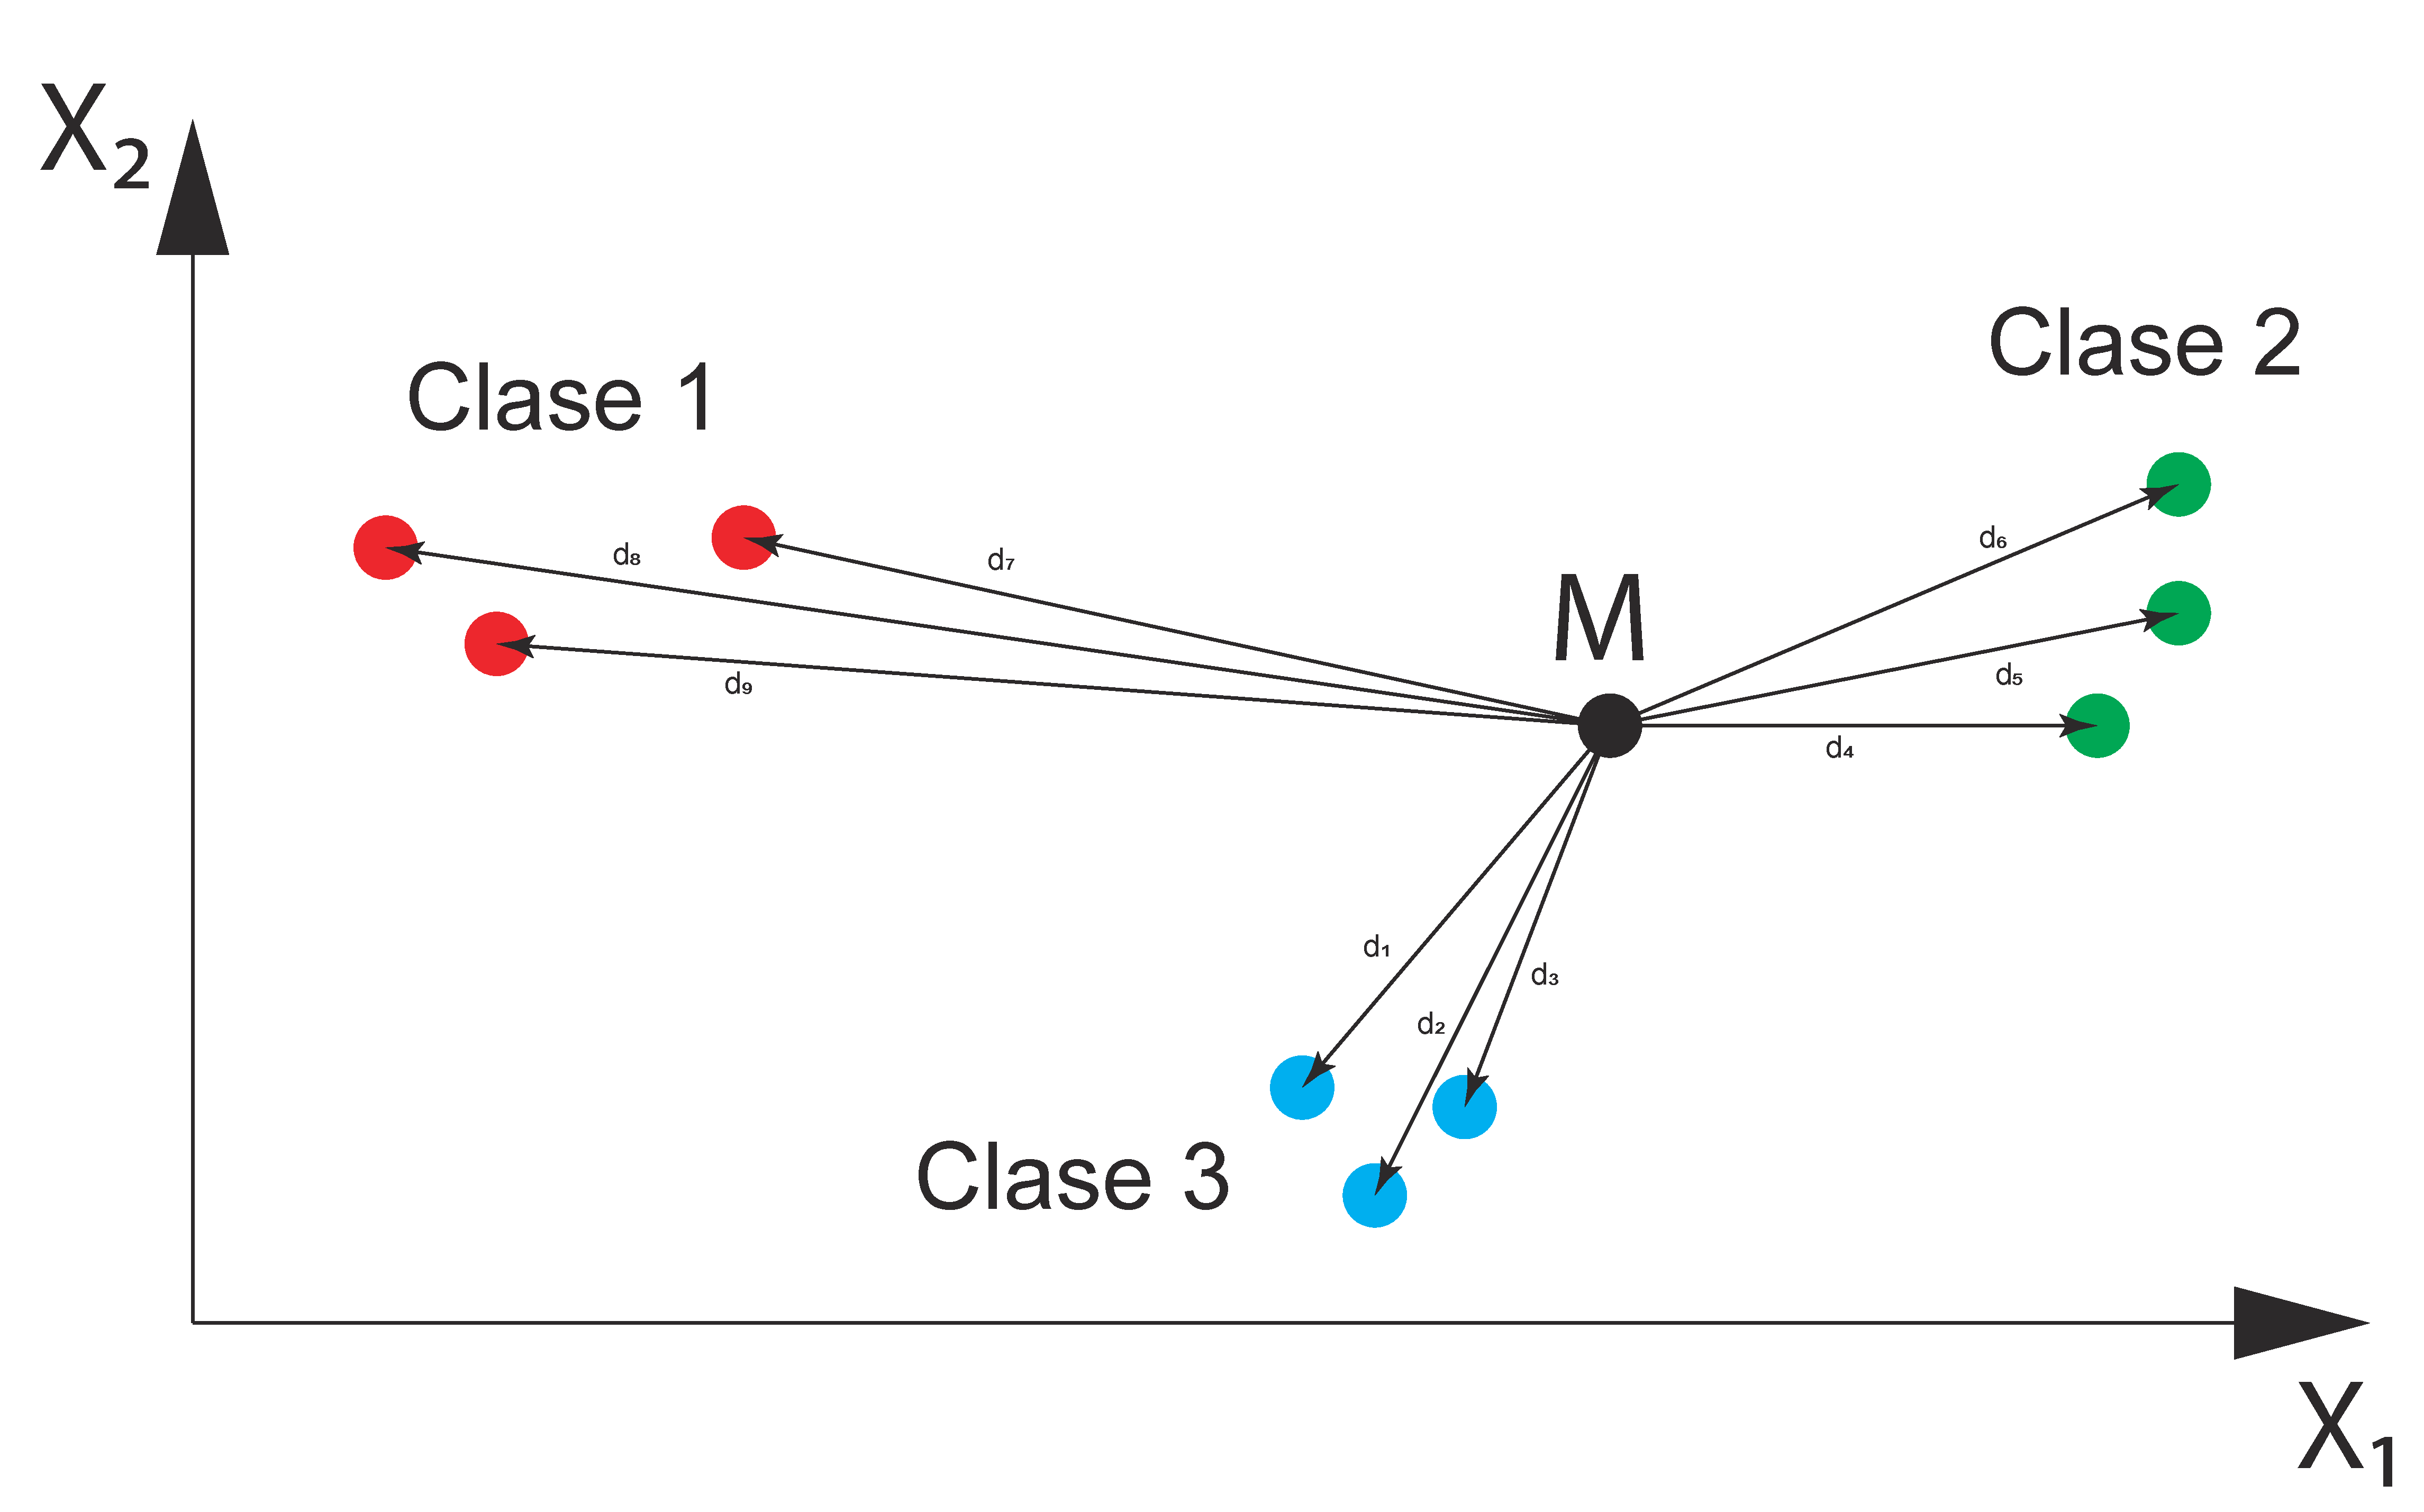
\includegraphics[width=\textwidth]{imagenes/marco_teorico/knn/knn_ejemplo1.pdf}
	\caption{Ejemplo clasificación Knn con datos bidimensionales (caso balanceado)}
	\label{fig:knn_ejemplo1}
\end{figure}

\begin{table}[H]
	\centering
	\caption{Ejemplo distancias clasificación knn}
	\label{tab:knn_distancias}
	\begin{tabular}{|c|c|}
		\hline
		Distancia & Clase \\ \hline
		$d_{1}$        & 3     \\ \hline
		$d_{2}$        & 3     \\ \hline
		$d_{4}$        & 2     \\ \hline
		$d_{3}$        & 3     \\ \hline
		$d_{5}$        & 2     \\ \hline
		$d_{6}$        & 2     \\ \hline
		$d_{7}$        & 1     \\ \hline
		$d_{8}$        & 1     \\ \hline
		$d_{9}$        & 1     \\ \hline 
	\end{tabular}
\end{table}

En función del parámetro $k$, la muestra $M$ será asignada a la clase más repetida de entre las $k$ menores distancias en la tabla \ref{tab:knn_distancias}. De ser $k = 4$, $M \rightarrow\:Clase\:3 $ pues, de las 4 mínimas distancias, la clase 3 tiene la mayor frecuencia.

\paragraph{Centroide más cercano} Existe una variación al método knn que se basa en calcular la distancia de la muestra M a los centroides de cada clase. Es decir, cada clase se representa como el centroide de todos sus puntos, a partir del cual se calcula la distancia con la muestra objetivo y se escoge la clase con la mínima distancia. La ventaja de este método es que no requiere ningún parámetro, sólo especificar el tipo de distancia a utilizar, sin embargo, no es una buena opción cuando las clases son no-convexas así como si presentan varianzas muy diferentes.

\paragraph{Knn con datos desbalanceados} El modelo knn no sufre con datos desbalanceados, sin embargo es posible implementar un peso por muestra invirtiendo su distancia, de tal forma que, a mayor distancia de la muestra,  menor influencia en el resultado.
\subsection{SVM}

Del inglés, \textit{Support Vector Machines}, SVM es un modelo de clasificación binaria supervisada que se basa en la aplicación de hiperplanos para separar las muestras de dos clases.

Suponiendo que se tiene un conjunto de datos de la forma $\left(X_{1},Y_{1}\right),\:\left(X_{2},Y_{2}\right),\:...,\:\left(X_{n},Y_{n}\right)$ siendo $Y_{n}$ la etiqueta de la clase a la que pertenece la muestra $X_{n}$ de la forma $\left(-1,1\right)$, con $X_{n}$ siendo un conjunto d-dimensional de $d$ características extraídas de la forma $\left(x_{1},x_{2},...,x_{d}\right)$ y una muestra a clasificar $S$ de la misma forma que $X_{n}$, el modelo SVM busca un hiperplano que separe los puntos $X_{n}$ con $Y_{n} = -1$ de los puntos con $Y_{n} = 1$.

Para ilustrar, de forma sencilla, el funcionamiento de los modelos SVM, se suponen dos clases de datos, $\left(1,-1\right)$, en un espacio de características bidimensional.

\begin{figure}[H]
	\centering
	\captionsetup{justification=centering}
	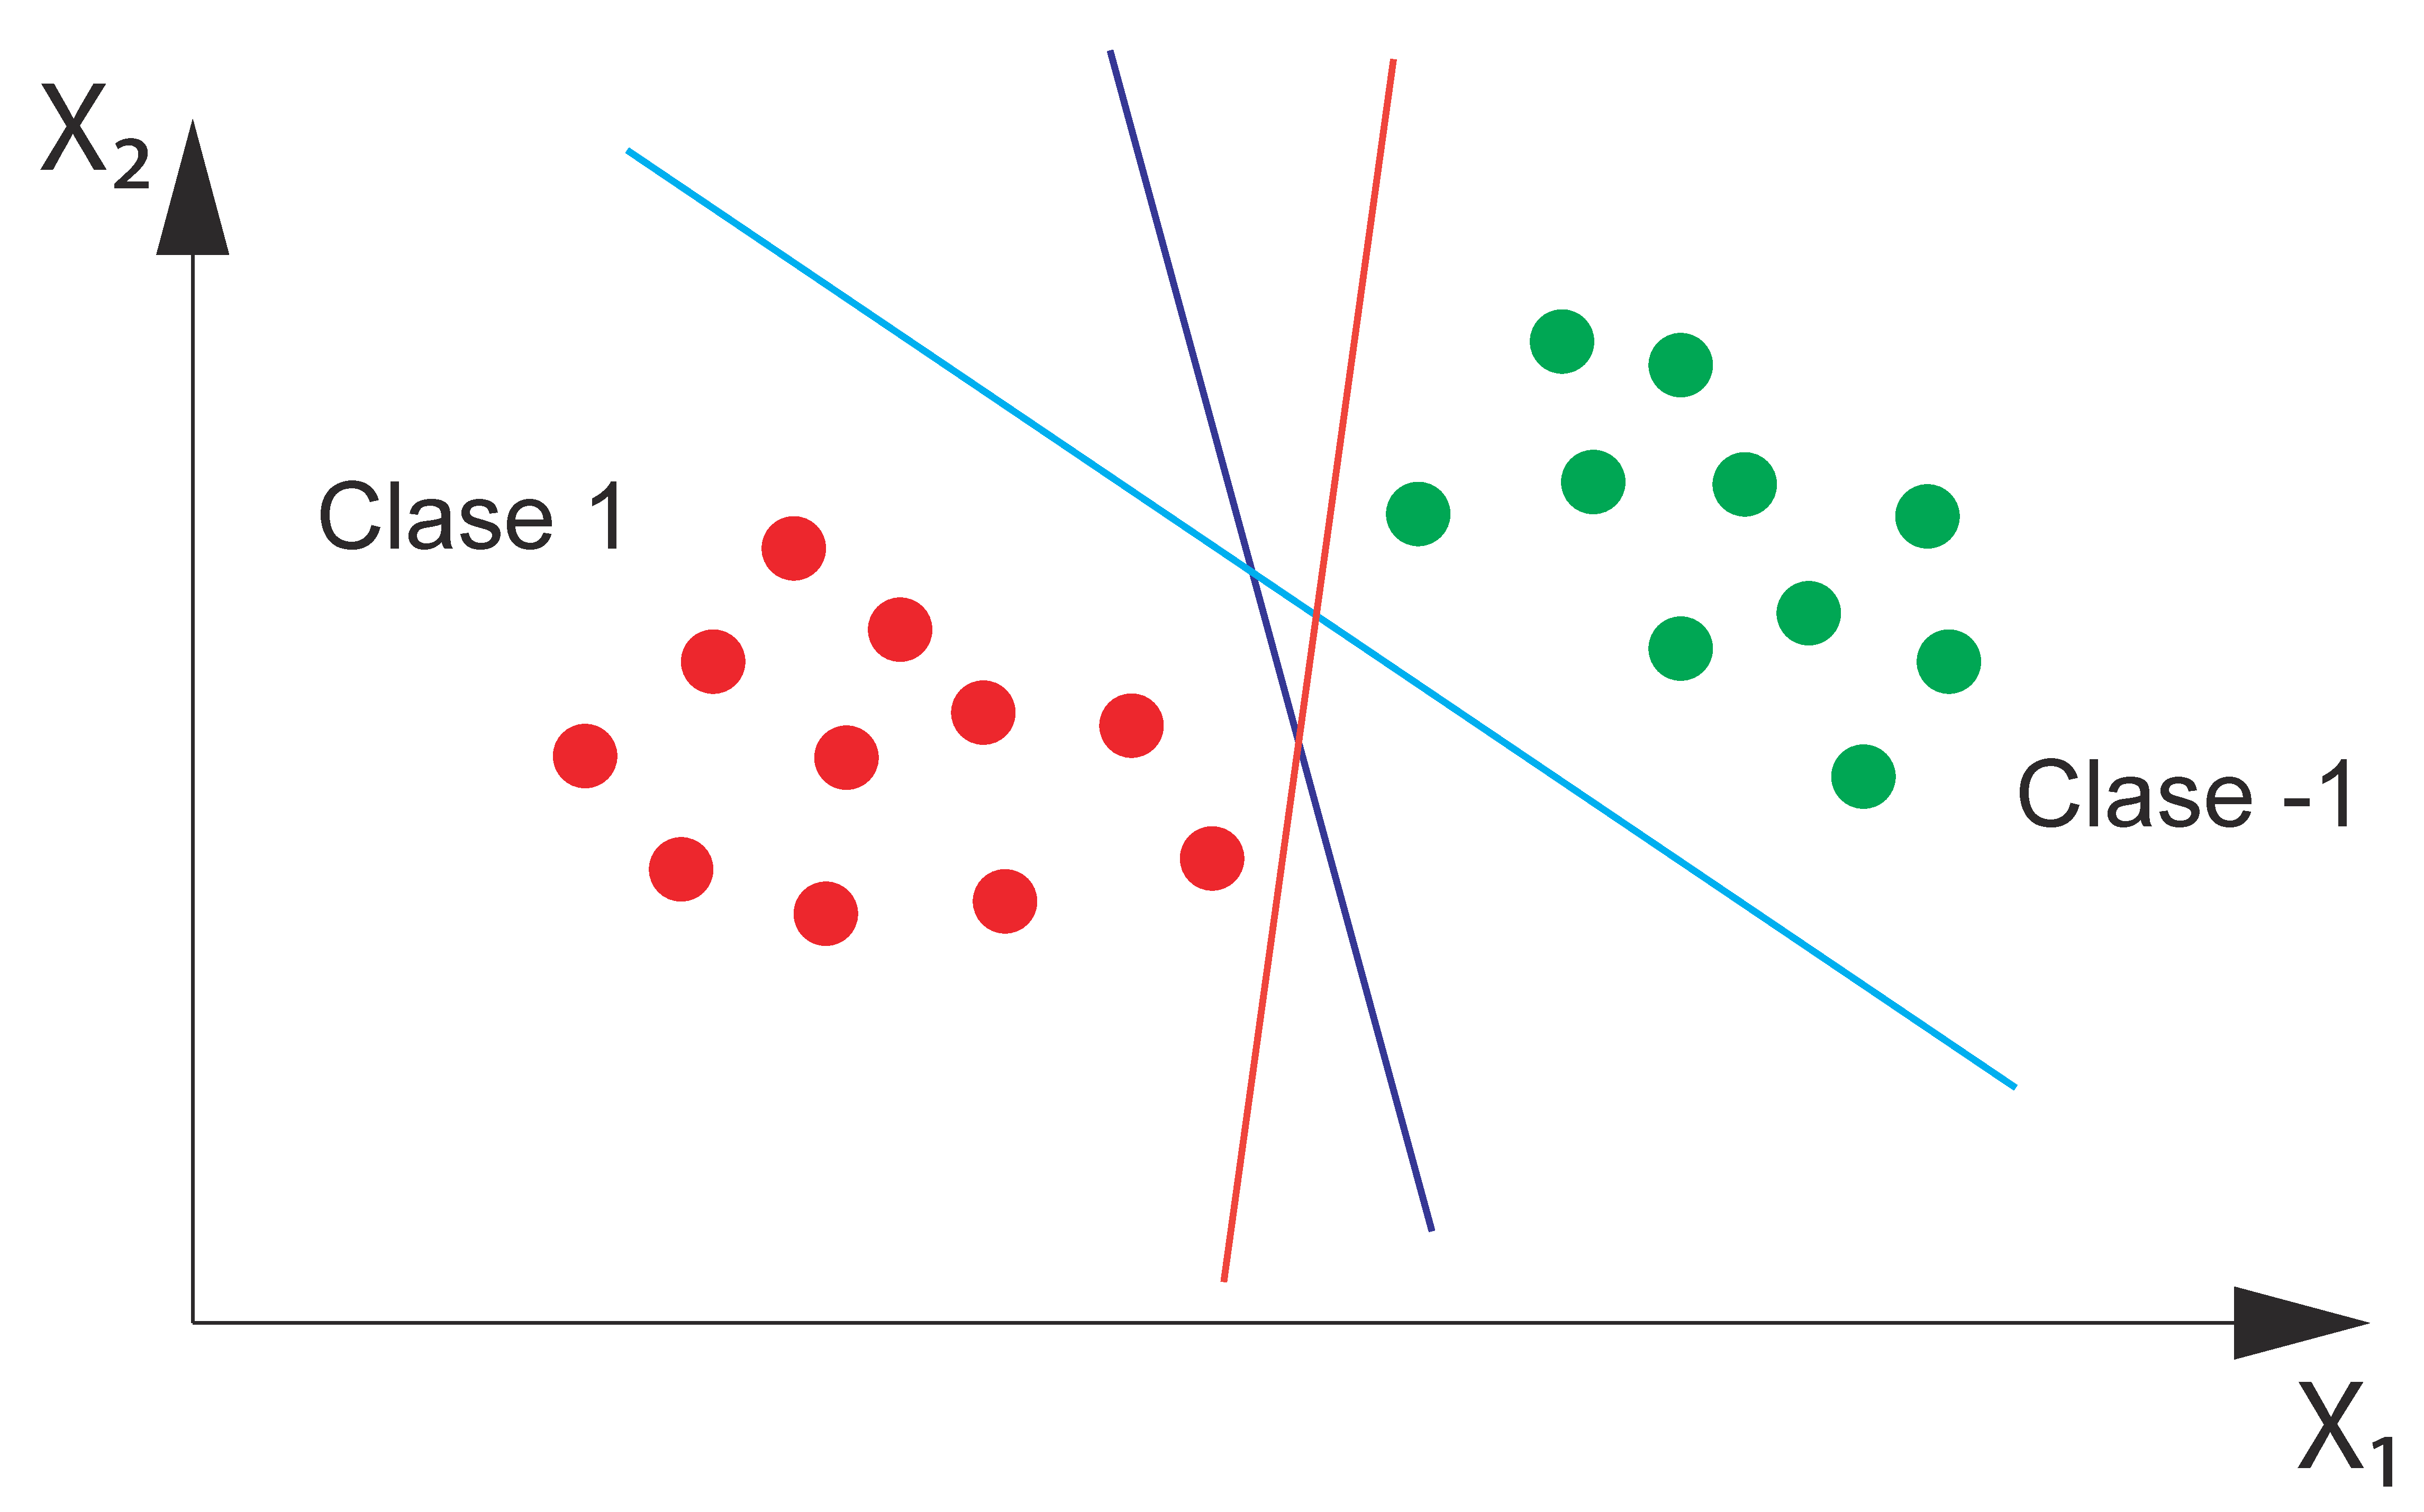
\includegraphics[width=\textwidth]{imagenes/marco_teorico/SVM/svm_ejemplo1.pdf}
	\caption{Ejemplo de SVM}
	\label{fig:svm_ejemplo1}
\end{figure}

La figura \ref{fig:svm_ejemplo1} muestra posibles hiperplanos (en dos dimensiones, un hiperplano es una recta) para clasificar a las dos clases. Cualquiera de las tres rectas mostradas es correcta, sin embargo, la mejor solución posible es aquella recta que maximice la distancia (maxímo margen) a ambas clases (veáse figura \ref{fig:svm_ejemplo2}).

\begin{figure}[H]
	\centering
	\captionsetup{justification=centering}
	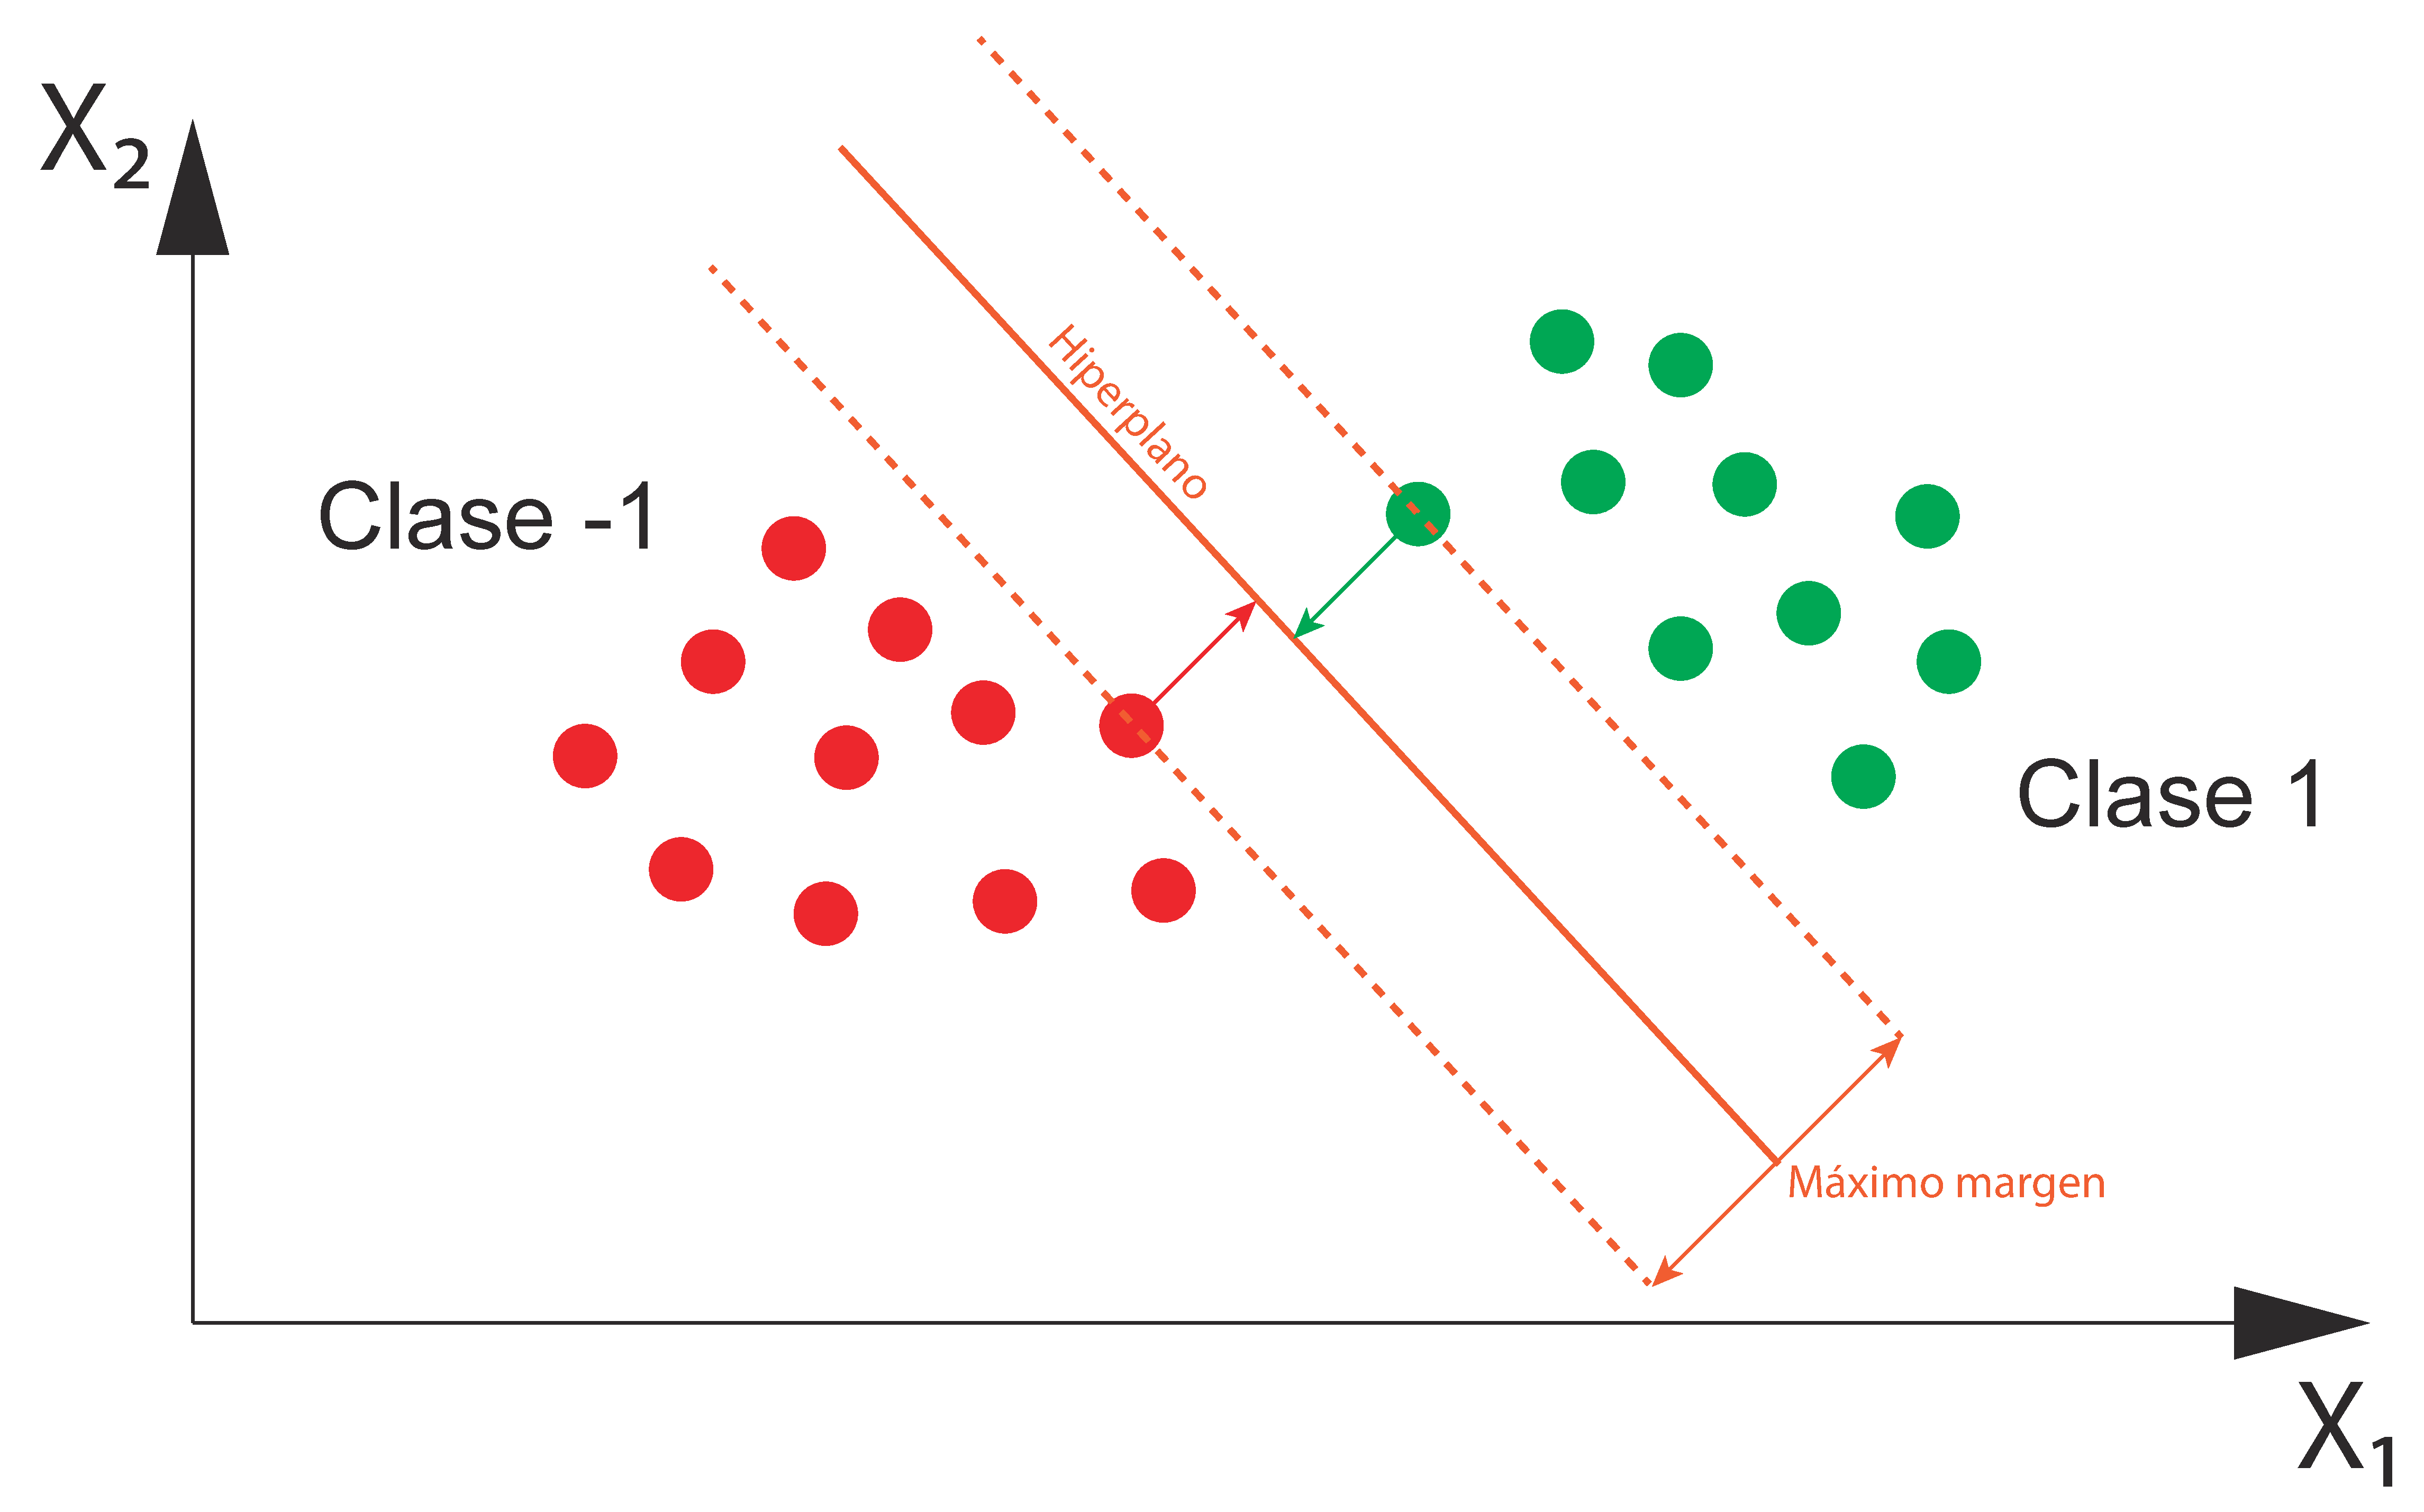
\includegraphics[width=\textwidth]{imagenes/marco_teorico/SVM/svm_ejemplo2.pdf}
	\caption{Recta óptima SVM}
	\label{fig:svm_ejemplo2}
\end{figure}

Matemáticamente, un hiperplano es definible como $w^{T}x-b=0$, siendo $w$ el vector normal al hiperplano y $\dfrac{b}{||w||}$ el desplazamiento del hiperplano respecto al origen en la dirección de $w$.

Existen dos posibles casos según las características de los datos:

\subsubsection{Datos linealmente separables}

En este caso, es posible definir dos hiperplanos adicionales de la forma $w^{T}x - b = 1$ (hiperplano superior al principal) y $w^{T}x - b = -1$ (hiperplano inferior al principal).

\begin{figure}[H]
	\centering
	\captionsetup{justification=centering}
	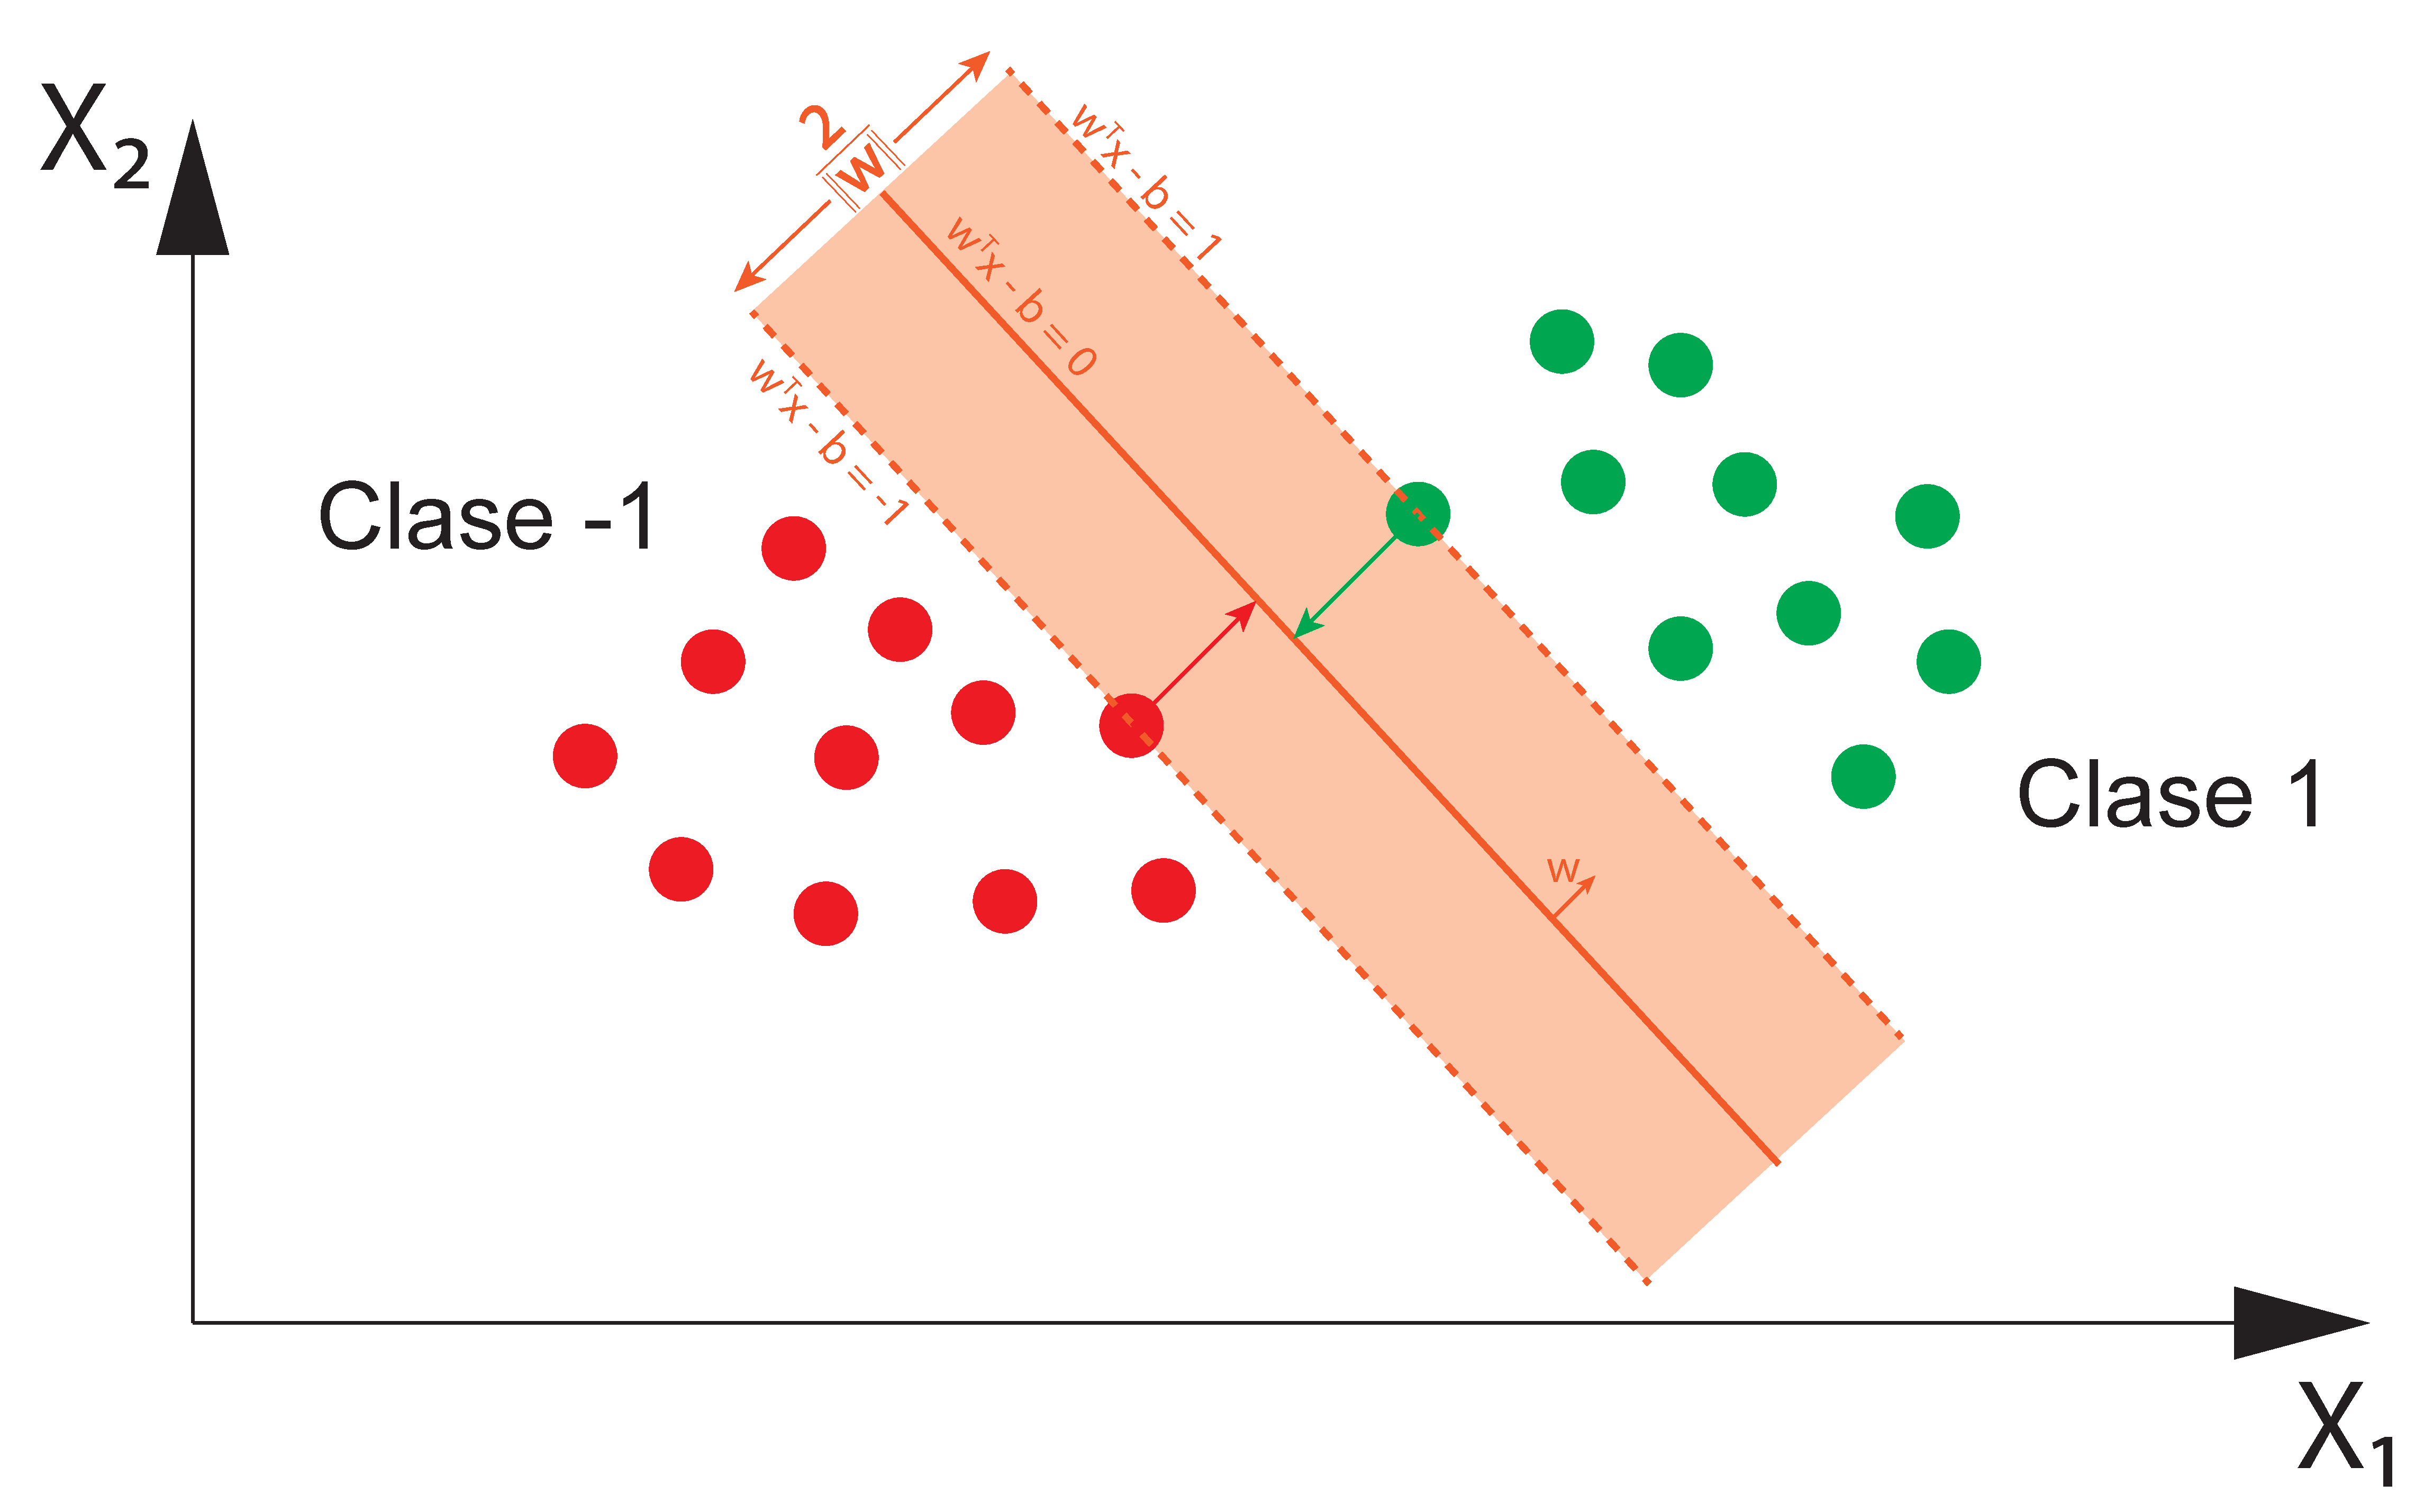
\includegraphics[width=\textwidth]{imagenes/marco_teorico/SVM/svm_ejemplo3.pdf}
	\caption{Hiperplanos adicionales SVM}
	\label{fig:svm_ejemplo3}
\end{figure}

La distancia entre los dos hiperplanos adicionales es $\dfrac{2}{||w||}$, por tanto, si se quiere maximizar el margen entre ambas rectas, se ha de minimizar $||w||$. Además, dado que ningún punto de ambas clases debe estar entre los dos hiperplanos, se pueden añadir dos condiciones:

\begin{description}
	\centering
	\item[] $w^{T}x_{i}-b\geq1,\:si\:y_{i}=1$
	\item[] $w^{T}x_{i}-b\leq1,\:si\:y_{i}=-1$
\end{description}

Reescribiendo ambas condiciones, se obtiene la expresión \ref{eqn:svm_condicion_lineal} y junto con la condición de minimizar $||w||$ se define el problema de optimización \ref{eqn:svm_hard_margin}:

\begin{equation}
	y_{i}\left(w^{T}x_{i}-b\right)\geq1,\: \forall\: 1\leq i\leq n
	\label{eqn:svm_condicion_lineal}
\end{equation}

\begin{equation}
	\mbox{Minimizar } ||w|| \mbox{ acorde a la condición } y_{i}\left(w^{T}x_{i}-b\right)\geq1,\: \forall\: 1\leq i\leq n
	\label{eqn:svm_hard_margin}
\end{equation}

\subsubsection{Datos linealmente inseparables}

Cuando los datos no son linealmente separables se utiliza la función de pérdida conocida como \textit{Hinge loss} (no tiene traducción formal al castellano) para minimizar el error.

\mynote{Una función de pérdida analiza cuánto se ha desviado la predicción del modelo frente al valor real.}

La función de pérdida es definida como:

\begin{equation}
	h(y) = max\left(0,1-t\cdot y\right)
	\label{eqn:svm_hinge_loss}
\end{equation}

La variable $t$ representa el valor real a determinar, mientras que $y$ es la predicción del clasificador. 

Comparando con la ecuación \ref{eqn:svm_condicion_lineal}, $t = w^{T}x_{i}-b = \pm 1$.

En el caso de que el clasificador prediga correctamente la clase, $y = t$, siendo $|y| = 1$ y, por tanto, la función de pérdida $h(y) = max(0,0) = 0$. Cuando la predicción no sea correcta, $y = -t$, la función de pérdida $h(y) = max(0,1-(-1)\cdot(1)) = max(0,2) = 2$. Es decir, $h(y)$ será nula cuando la predicción sea correcta.

Esto significa que la función de pérdida $h(y)$ será nula cuando $x_{i}$ se encuentre en el lado correcto del hiperplano y fuera del margen. 

Para los puntos que no puedan clasificarse y su error sea permitido, se introduce la variable $\zeta_{i}$ para $x_{i}$, que no es sino la función \ref{eqn:svm_hinge_loss} evaluada para $x_{i}$. Además, se define un parámetro de regularización, $C$, que controla el maximizar el margen contra minimizar el error. Es decir, para elevados valores de C, el problema de optimización determinará un hiperplano con los márgenes mínimos posibles para poder abarcar todos los puntos posibles (minimizar los puntos mal clasificados); para valores reducidos de C, el optimizador buscará un hiperplano con márgenes más amplios, aunque cometa el error de clasificar erróneamente más puntos.

Por tanto, para los puntos "fuera de posición", el error se define como:

\begin{equation}
	C\sum_{i=1}^{n} \zeta_{i} = C\sum_{i=1}^{n} max\left(0,1-t\cdot y\right)
	\label{eqn:svm_error_soft_margin}
\end{equation}

De tal forma, ahora el problema de optimización es:

\begin{equation}
	\begin{split}
		\mbox{Minimizar } \dfrac{1}{2} ||w||^{2} + C\sum_{i=1}^{n} max\left(0,1-t\cdot y\right) \\	
		\mbox{ acorde a la condición } y_{i}(w^{T}x_{i}-b)\geq 1-\zeta_{i},\: \forall\: 1\leq i\leq n
	\end{split}
	\label{eqn:svm_soft_margin}
\end{equation}

\paragraph{Parámetro $\nu$} INSERTAR CITA proponen el parámetro $\nu$ como alternativa a C, que representa un límite superior en la fracción de errores de margen y un límite inferior de la fracción de vectores de soporte. Es decir, el valor de $\nu$ determina el máximo de muestras a ser mal clasificadas (fuera de márgenes) y el número mínimo de muestras que serán vectores de soporte. $C$ y $\nu$ se relacionan de la forma $\nu = \dfrac{c_{1}c_{2}}{C}$ siendo $c_{1}$ y $c_{2}$ constantes a calcular por el optimizador.

\subsubsection{Problema dual}

De acuerdo al Teorema de la Dualidad, es posible ver el problema de optimización definido por \ref{eqn:svm_hard_margin} (conocido como problema primitivo) desde otra perspectiva (problema dual).

Utilizando el método de los multiplicadores de Lagrange, se puede definir la ecuación \ref{eqn:svm_hard_margin} como \ref{eqn:svm_lagrange_multiplicadores}, a partir de la cual el problema de optimización se define como \ref{eqn:svm_lagrange_optimizacion}. Por un lado se busca encontrar el valor de $w,b$ que minimice el valor de \ref{eqn:svm_lagrange_multiplicadores} para cada $\alpha_{i}$ y escoger, de entre todos los $\alpha_{i}$, el valor máximo.

\begin{equation}
	\mathcal{L}(w,b,\alpha) = \dfrac{1}{2}||w||^{2}	- \sum_{i=1}^{n}\alpha_{i}(y_{i}((w^{T}x_{i}-b)-1)
	\label{eqn:svm_lagrange_multiplicadores}
\end{equation}

\begin{equation}
	\mbox{MAX}_{\alpha_{i}\geq0}\left[\mbox{MIN}_{w,b}\:\mathcal{L}(w,b,\alpha)\right]
	\label{eqn:svm_lagrange_optimizacion}
\end{equation}

La resolución de \ref{eqn:svm_lagrange_optimizacion} se consigue derivando parcialmente $\mathcal{L}$ respecto de $w$ y de $b$:

\begin{equation}
	\begin{split}
		\dfrac{\partial \mathcal{L}}{\partial w} = 0 \rightarrow w = \sum_{i=1}^{n} \alpha_{i}y_{i}x_{i} \\
		\dfrac{\partial \mathcal{L}}{\partial b} = 0 \rightarrow \sum_{i=1}^{n} \alpha_{i}y_{i} = 0 = \alpha_{T}y \\
	\end{split}
	\label{eqn:svm_derivadas_lagrange}
\end{equation}

Para facilitar el cálculo, para los $x_{i}$ que no sean vectores soporte (a partir de ahora SV), sus multiplicadores de Lagrange $\alpha_{i} = 0$.

De tal forma, si se sustituye \ref{eqn:svm_derivadas_lagrange} en \ref{eqn:svm_lagrange_optimizacion} se obtiene la expresión de optimización para un clasificador SVM de la forma dual:

\begin{equation}
	\mbox{MIN}_{\alpha_{i}\geq0} \left[\sum_{i=1}^{n}\alpha_{i} - \dfrac{1}{2}\sum_{i,j}\alpha_{i}\alpha_{j}y_{i}y_{j}x_{i}^{T}x_{j}\right]
	\label{eqn:svm_dual}
\end{equation}

\mynote{En la ecuación superior, $(i,j)$ representan cada clase del problema.}

Tanto la resolución del problema dual como la del primitivo permiten obtener las soluciones del otro (propiedad del Teorema de la Dualidad). Sin embargo, optimizar el SVM mediante \ref{eqn:svm_dual} permite hacer uso de Kernels.

\subsubsection{Aplicación de kernels en SVM}

En muchas aplicaciones, los datos a clasificar pueden no parecer ser linealmente separables. Véase, por ejemplo, la figura %%%%%%.

\imagetest

Un conjunto de datos $X \epsilon\: \rm I\!R^{n}$ puede ser no separable con hiperplanos en dimensión $n$. Sin embargo, para una dimensión $m$, tal que $m > n$, $X$ si es separable. De tal forma, se puede definir una función $\phi:\: \rm I\!R^{n}\: \rightarrow\: \rm I\!R^{m}$, que transforme los datos de un espacio dimensional $n$, donde no sean separables linealmente, a un espacio dimensional superior $m$ donde si lo sean.

Haciendo referencia al problema dual, en la ecuación \ref{eqn:svm_dual}, segundo término, se presenta la multiplicación escalar de $x_{i}^{T}x_{j}$ para el espacio dimensional original $\rm I\!R^{n}$. Esta expresión se entiende, a \textit{grosso modo}, como que el clasificador SVM va a aprender de los datos en la dimensión $n$. 

Si se da el casos de datos no lineales en $n$, pero si en $m$, el clasificador tendría que "aprender" de los datos en la dimensión $n$ y, por tanto, sería necesario calcular los valores de $X$ en $\rm I\!R^{m}$. Si $m$ es muy elevado, esto es computacionalmente muy pesado, haciendo que sea una gran desventaja.

La aplicación de un kernel permite evitar tener que calcular la representación de $X$ en $\rm I\!R^{m}$, es decir, evita que el clasificador tenga que "aprender" de los valores en la dimensión superior, haciendo que sólo haga falta conocer el resultado del producto vectorial en $\rm I\!R^{m}$.

Un kernel $k(x_{1},x_{2})$ es una función que, bajo las condiciones del Teorema de Mercer, puede expresarse como una multiplicación escalar $<\phi(x_{1}),\phi(x_{2})>$, siendo $\phi:\: \rm I\!R^{n}\: \rightarrow\: \rm I\!R^{m}$.

Se define, por ejemplo, el kernel $k(x,x') = (x^{T}x')^{3}$, con $x,x'\:\epsilon\: \rm I\!R^{2}$, que resuelve el producto escalar de $x$ y $x'$ en $\rm I\!R^{4}$ usando sus formas en $\rm I\!R^{2}$, sin necesidad de calcular los valores de $x,x'$ en $\rm I\!R^{4}$ y realizar la multiplicación escalar en tal dimensión.

\begin{equation}
	\centering
	\begin{gathered}
		k(a,b) = (a^{T}b)^{3}
		= ((a_{1},a_{2})^{T}(b_{1},b_{2}))^{3} \\
		= (a_{1}b_{1}+a_{2}b_{2})^{3} \\
		= a_{1}^{3}b_{1}^{3} + 3a_{1}^{2}b_{1}^{2}a_{2}b_{2} + 3a_{1}b_{1}a_{2}^{2}b_{2}^{2} + a_{2}^{3}b_{2}^{3} \\
		= (a_{1}^{3},\sqrt{3}a_{1}^{2}a_{2},\sqrt{3}a_{1}a_{2}^{2},a_{2}^{3})^{T}\:(b_{1}^{3},\sqrt{3}b_{1}^{2}b_{2},\sqrt{3}b_{1}b_{2}^{2},b_{2}^{3}) \\
		= \phi(a)\cdot\phi(b)		
	\end{gathered}
	\label{eqn:svm_kernel_ejemplo}
\end{equation}

Gracias a \ref{eqn:svm_kernel_ejemplo}, se ha obtenido el resultado de la multiplicación escalar $\langle \phi(x_{1}),\phi(x_{2})\rangle$, sin necesidad de transformarlos a $\rm I\!R^{4}$, haciendo uso de sus formas en $\rm I\!R^{2}$, ahorrando el tiempo y cálculo necesario para ello.

De entre la gran cantidad de kernels ya definidos y los definibles por el usuario, se destacan los que serán usados más adelante en la implementación:

\begin{itemize}
	\item Kernel lineal 
		\begin{equation}
			k(x_{1},x_{2}) = \langle x_{1},x_{2}\rangle
			\label{eqn:svm_kernel_lineal}
		\end{equation}	
	\item Kernel polinómico 
		\begin{equation}
			k(x_{1},x_{2}) = (\gamma\langle x_{1},x_{2}\rangle+r)^{d}
			\label{eqn:svm_kernel_poly}
		\end{equation}
	\item Kernel RBF
		\begin{equation}
			k(x_{1},x_{2}) = e^{-\gamma||x_{1}-x_{2}||^{2}}
			\label{eqn:svm_kernel_rbf}
		\end{equation}
	\item Kerngel Sigmoid 
		\begin{equation}
			k(x_{1},x_{2}) = tanh(\gamma\langle x_{1},x_{2}\rangle+r)
			\label{eqn:svm_kernel_sigmoid}
		\end{equation}
\end{itemize}

\subsubsection{Clasificación multiclase con SVM}

Debido al uso de hiperplanos, los modelos SVM sólo son capaces de clasifican binaria. Si se requiere su uso para la clasificación de más de dos clases, es necesario elegir entre dos estrategias:

\paragraph{Clasificación Uno contra Todos} \label{par:OVR}

Abreviada como OVR (del inglés \textit{One vs Rest}), el método de uno contra todos convierte una clasificación multiclase a binaria considerando la clase objetivo como la clase positiva (1) y las clases restantes como negativas (0). Sin embargo, requiere entrenar un clasificador por clase. Para un caso de $N$ clases, se requiere de $N$ clasificadores.

\paragraph{Clasificación Uno contra Uno} \label{par:OVO}

Abreviada como OVO (del inglés \textit{One vs One}), el método de uno contra uno convierte una clasificación multiclase a binaria considerando una clase como positiva (1) y entrenando un clasificador para cada clase restante, considerada como negativa (0). Este planteamiento requiere entrenar $\dfrac{N(N-1)}{2}$ clasificadores, muchos más que con OVR, haciéndolo más lento y computacionalmente más pesado. Sin embargo, su gran ventaja es que, para métodos de clasificación (SVM y otros métodos) que sufran con grandes cantidades de datos, OVO solo clasifica entre dos clases, lo que implica clasificar muchas menos muestras en vez de la totalidad de ellas (OVR).

% https://www.cs.toronto.edu/~urtasun/courses/CSC411_Fall16/16_svm.pdf



